\newcommand{\institut}{Institut f\"ur Telekommunikationssysteme}
\newcommand{\fachgebiet}{Nachrichten\"ubertragung}
\newcommand{\veranstaltung}{Praktikum Nachrichten\"ubertragung}
\newcommand{\pdfautor}{Dirk Babendererde (321 836), Thomas Kapa (325 219)}
\newcommand{\autor}{Dirk Babendererde (321 836)\\ Thomas Kapa (325 219)}
\newcommand{\gruppe}{Gruppe:}
\newcommand{\betreuer}{Betreuer: Lieven Lange}


\newcommand{\pdftitle}{Nachrichtenuebertragung\ Praktikum\ 03}
\newcommand{\prototitle}{Praktikum 03 \\ Statistische Nachrichtentheorie}

\input{../../packages/tu_header_9}


%     \lstinputlisting{./praktikum6.sce}

%---------------------------------------------------------------------
%---------------------------------------------------------------------
%---------------------------------------------------------------------


\section{Vorbereitungsaufgaben}
\begin{quote}
    \hspace{-2em}
    \subsection{AM}
        
    \begin{quote}
        
        Da alle Werte eines analogen Signals $\geq 0$ sein Müssen um sie mittels AM mit Träger übertragen zu können, haben wir für
        diesen Versuch mit Matlab Cosinus-, Dreieck- und Rechtecksignale folgenden Eigenschaften erzeugt:
        
        
        \begin{equation*}
        \begin{split}
        \\
                 0 &\leq u(t) \leq 2.0
        \\
                 f &= \si{100}{Hz}
        \\
            \alpha &= 0.5
        \\
                 T &= \si{2}{s}
        \\
               f_T &= \si{1}{MHz}
        \\
        \end{split}
        \end{equation*}
        
        
        Außerdem haben wir noch ein cosinus-Trägersignal mit \si{2}{kHz} erzeugt. Auf dieses Trägersignal haben wir dann, zum
        späteren vergleich, die erzeugten Basisbandsignale raufmoduliert.
        
    \end{quote}
    
    
    
    
    \subsection{FM}
    \begin{quote}
        
        
        Zur Vorbereitung der FM-Modulation haben wir ein Cosinussignal mit folgenden Eigenschaften simuliert.
        
        \begin{equation*}
        \begin{split}
        \\
                 0 &\leq u(t) \leq 2.0
        \\
                 f &= \si{100}{Hz}
        \\
                 T &= \si{0,5}{s}
        \\
               f_T &= \si{1}{MHz}
        \\
        \end{split}
        \end{equation*}
        
        
        Dieses Trägersignal haben wir dann mit einem weiteren cosinus ($f_u = 1kHz$ und $A_u = 1V$) nach der folgenden Formel
        moduliert:
        
        \begin{equation*}
        \begin{split}
        \\
                u_m(t) &= A \p cos(\varphi(t))
        \\
            \varphi(t) &= 2 \pi f_c t + K_{FM} \p \int\limits_{-\infty}^t u(\tau) \ d\tau  
        \\
        \end{split}
        \end{equation*}
        \label{equ:fm}
        
        Von diesem Modulierten Signal ($u_m$) haben wir noch, zum späteren Vergleich, mit Hilfe von Matlab das Amplitudenspektrum
        bestimmt.
        
        
    \end{quote}
    
    
    \subsection{Theorie zur FM-Demodulation}
    \begin{quote}
        
        Die grundlegende Abfolge der Verwendeten FM-Demodulation ist wie Folgt:\\
        \vspace{0.1em}
        
        \begin{itemize}
          \item Wir starten mit einem modulierten Signal, bei dem die Frequenz proportional steigt wenn das Nutzsignal positiv war
                und bei negativen werten des Eingangssignals wieder sinkt.
          \item Aus diesem Signal wird (z.B. per Comparator und Pulsgenerator) nach jeder Periode (idealer weise) ein Deltaimpuls
                erzeugt.
          \item Diese Pulsvolge wird anschließend Tiefpassgefiltert, was sich gut anhand eines CR-Gliedes (C-in Reihe, R-Paralel)
                erklären lässt.
          \item Der kondensator läd sich bei kleineren Abständen der Pulse schneller auf als er siche wieder entläd und bei
                größeren Abständen entläd er sich schneller als er sich aufläd.
          \item Damit steigt die Spannung über dem Kondensator für kürzere abstände der Nulldurchgänge (also höhere Frequenzen)
                und sie sinkt für kleinere Abstände (also niedrigere Frequenzen).\\
        \end{itemize}
        
        \vspace{-1em}
        Dieses Verhalten ist das exakte gegenteil der modulation und extrahiert somit das Nutzsignal wieder aus dem Träger.
        
        
    \end{quote}
    
    
\end{quote}

%--------------------------------------------------------------------
%--------------------------------------------------------------------


\section{AM}
\begin{quote}
    
    
    \subsection{Labordurchführung}
    \begin{quote}
      Das mit Hilfe von Amplitudenmodulation zu übertragende Signal soll ein
      Sinussignal mit Amplitude von 1 V, einer Frequenz von 100 Hz, mittelwertfrei sein und von Funktionsgenerator geliefert 
      werden. Um das Signal von negativen Werten zu befreien (siehe
      Vorbereitung) wird das Signal mit Hilfe des Adder-Moduls und der variablen DC Voltage Quelle
      um ein Volt angehoben. Da das Adder-Modul den Ausgang invertiert, wird der
      Ausgang des ersten Adders auf einen zweiten Adder gegeben und der zweite
      Eingang auf Masse gelegt, um das Signal zu invertieren.
      Um Trägersignal und das zu übertragende Signal zu überlagern wird das
      Multiplier-Modul verwendet. Dabei liefert das Master-Signal-Modul ein 2
      kHz Sinussignal, das als Trägersignal dient, das mit dem zu übertragenden
      Signal multipliziert wird.
        Mit der Demodulation über einen als idealen betrachteten Kanal kann das
        Signal durch eine erneute Multiplikation mit dem Trägersignal
        zurückgewonnen werden.
        
      \begin{equation*}
        \begin{split}
         y_{d}(t)=u_{m}(t)cos(\omega_{c}t)=u(t)cos^{2}(\omega_{c}t)=\frac{1}{2}u(t)\cdot
         (1+cos(2\omega_{c}t))
         \label{eq:demodulation}
        \end{split}
        \end{equation*}
        
        In Formel \ref{eq:demodulation} kann man erkennen, dass der vordere Teil
        bis auf den Vorfaktor 0,5 dem Basisbandsignal entspricht. Der hintere
        Teil weist eine doppelt so hohe Frequenz auf, die man mit einem
        entsprechend dimensionierten Filter herausfiltern kann.
        Dabei werden auch die Signale nach der Demodulation ohne Tiefpass
        aufgenommen und in der Auswertung mit denen mit Tiefpass verglichen.
        In Formel \ref{eq:demodulation} kann man weiterhin erkennen, dass das
        modulierte Signal zum einen aus dem Trägersignal mit seiner Frequenz und
        dem Nutzsignal und seiner Frequenz besteht und dies im
        Amplitudenstprektrum auch zu erwarten ist.\\
        Zuletzt kann man ein
        zweites Multiplier-Modul hinzufügen und den Ausgang von diesem auf einen entsprechenden Tiefpass geben und erhält sein Signal zurück.
        
    \end{quote}
    
    
    \subsection{Auswertung}
    \begin{quote}
        Eine Veränderung der Amplitude des Basisbandsignals führt dazu, dass,
        wenn die Amplitude zu groß wird, das Signal Anteile unter 0 bekommt.
        Damit verändert sich die Einhüllende des modulierten Signals und eine
        Rückgewinnung durch Demodulation ist nicht mehr möglich. Ein Beispiel
        ist in Abb. \ref{fig:Ampl} zu sehen, wobei die Amplitude bei 2 V liegt
        und der Offset bei 1 V.
        
    \begin{figure}[H]
		\begin{center}
			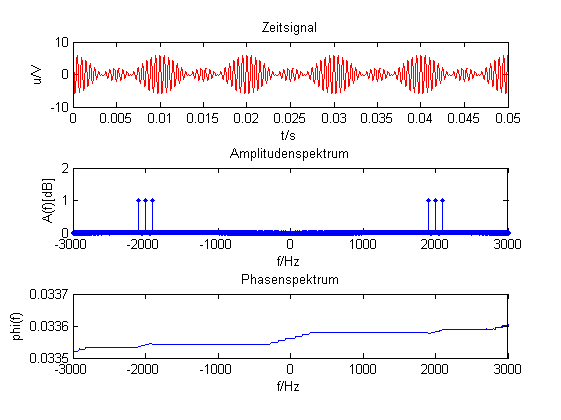
\includegraphics[width=0.8\textwidth]{Bilder/Cos_zugrosseAmpl}
		\end{center}
		\caption{zu große Amplitude des Basisbandsignals}
		\label{fig:Ampl}
	\end{figure}
	
	Bei dem Offset entsteht der selbe Fehler, nur dass dieser nicht zu klein
        sein darf. Abb. \ref{fig:Offs} zeigt die Modulation für eine Amplitude
        von 1 V und einem Offset von 0,2 V.
	
	 \begin{figure}[H]
		\begin{center}
			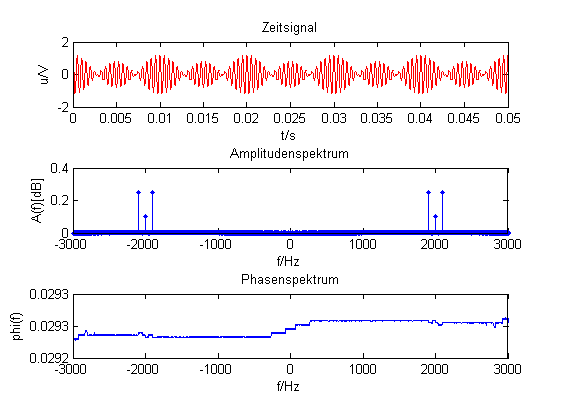
\includegraphics[width=0.8\textwidth]{Bilder/Cos_zukleinerOffset}
		\end{center}
		\caption{zu kleiner Offset des Basisbandsignals}
		\label{fig:Offs}
	\end{figure}
        
        In Abb. \ref{fig:Mocosinussimu} und \ref{fig:Mocosinus} sind sowohl die
        mit Matlab simulierte, als auch die gemessene Modulation eines Cosinus
        abgebildet. Es ist gut zu erkennen, dass die Simulation mit der Praxis
        gut übereinstimmen. Lediglich bei der Amplitude sind versehentlich
        unterschiedliche Werte aufgenommen worden.
        Gut zu erkennen sind jeweils die beiden großen Peaks bei +- 2 kHz des
        Trägersignals und die jeweils um diese 2 kHz um 100 Hz versetzten
        Nebenpeaks des Basisbandsignals, wie es von der Theorie erwartet wurde.  
        
        \begin{center}
        \begin{tabular}{ll}
        
        \hspace{-5cm}
            \begin{minipage}{0.67\textwidth}
                
                \begin{figure}[H]
                    \label{fig:Mocosinussimu}
                    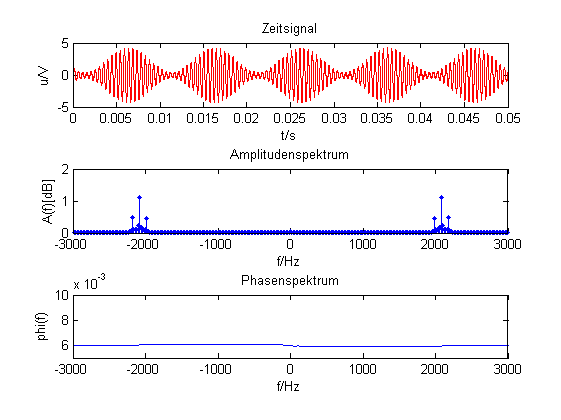
\includegraphics[scale=0.7]{Bilder/Am_Cos_2k_100Hz_mo_simu}
                    \caption{mit Matlab simulierte Modulation eines Cosinus}
                \end{figure}
        
            \end{minipage}
        
            \begin{minipage}{0.67\textwidth}
                \begin{figure}[H]
                    \label{fig:Mocosinus}
                    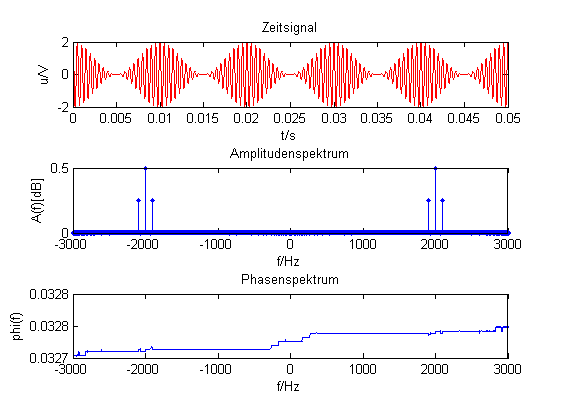
\includegraphics[scale=0.7]{Bilder/Am_Cos_2k_100Hz_mo}
                    \caption{gemessene Modulation eines Cosinus}
                \end{figure}
        
            \end{minipage}
        
        \end{tabular}
        \end{center}
        
        \begin{center}
        \begin{tabular}{ll}
        
        \hspace{-5cm}
            \begin{minipage}{0.67\textwidth}
                
                \begin{figure}[H]
                    \label{fig:Modreiecksimu}
                    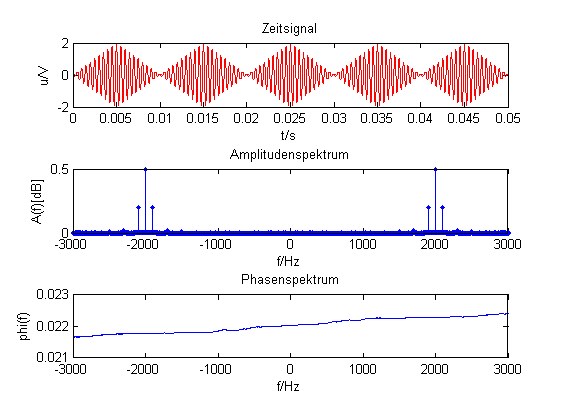
\includegraphics[scale=0.7]{Bilder/Am_Dre_2k_100Hz_mo_simu}
                    \caption{mit Matlab simulierte Modulation eines
                    Dreieck}
                \end{figure}
        
            \end{minipage}
        
            \begin{minipage}{0.67\textwidth}
                \begin{figure}[H]
                    \label{fig:Modreieck}
                    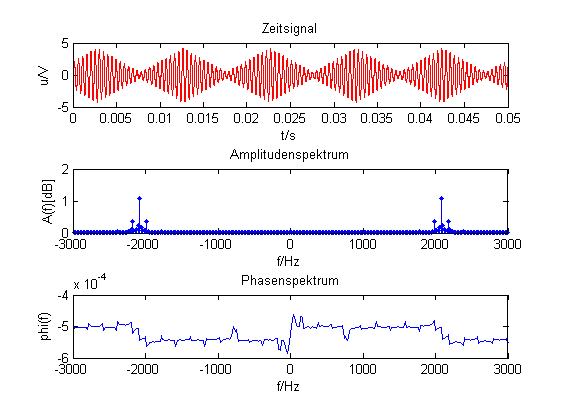
\includegraphics[scale=0.7]{Bilder/Am_Dre_2k_100Hz_mo}
                    \caption{gemessene Modulation eines Dreieck}
                \end{figure}
        
            \end{minipage}
        
        \end{tabular}
        \end{center}
      
        \begin{center}
        \begin{tabular}{ll}
      
        \hspace{-5cm}
            \begin{minipage}{0.67\textwidth}
                
                \begin{figure}[H]
                    \label{fig:Morechtecksimu}
                    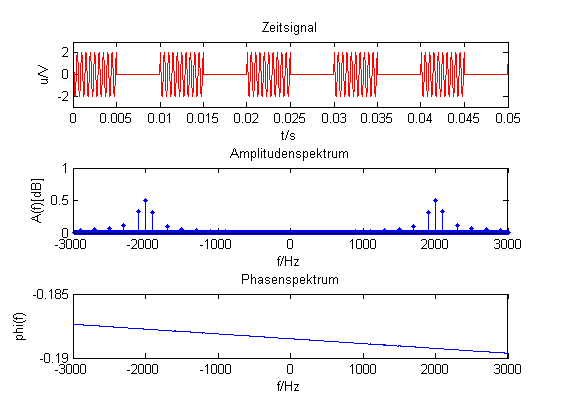
\includegraphics[scale=0.7]{Bilder/Am_Rec_2k_100Hz_mo_simu}
                    \caption{mit Matlab simulierte Modulation eines Rechteck}
                \end{figure}
        
            \end{minipage}
    
            \begin{minipage}{0.67\textwidth}
                \begin{figure}[H]
                    \label{fig:Morechteck}
                    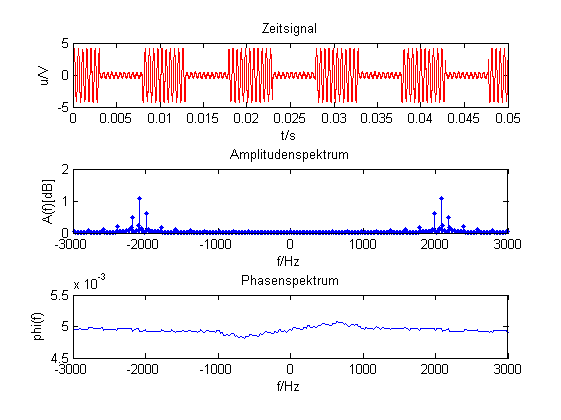
\includegraphics[scale=0.7]{Bilder/Am_Rec_2k_100Hz_mo}
                    \caption{gemessene Modulation eines Rechteck}
                \end{figure}
        
            \end{minipage}
        
        \end{tabular}
        \end{center}
        
        In Abb. \ref{fig:Sprache} ist die Modulation eines Sprachsignals zu
        sehen. Hierbei ist gut zu erkennen, dass die Nebenpeaks um die 2 kHz
        nicht den 100 Hz entsprechen, wie bei den ersten drei Signalen. Da ein
        Sprachsignal in einem breiteren Bereich von bis zu vier kHz liegt,
        streut das Sprektum hier mehr um die 2 kHz.
        
    \begin{figure}[H]
		\begin{center}
			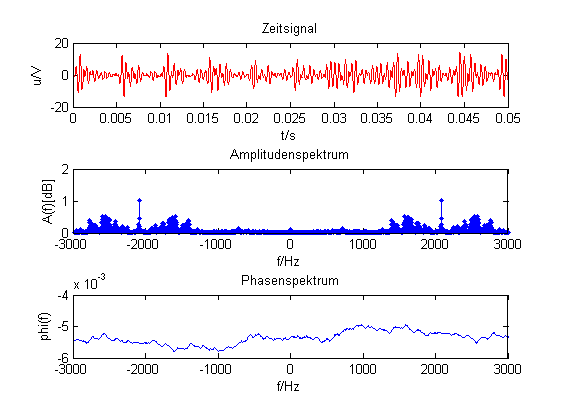
\includegraphics[width=0.8\textwidth]{Bilder/Sprachsignal}
		\end{center}
		\caption{Modulation eines Sprachsignals}
		\label{fig:Sprache}
	\end{figure}
        
        Bei der Demodulation werden zuerst die Signale ohne Tiefpass betrachtet.
        Dabei ergibt sich bei der Multiplikation mit dem selben Cosinus ein
        Cosinus Quadrat. Daher werden alle negativen Anteile nach oben geklappt
        und es gibt nur noch positive Anteile. Es sind auch noch mehrere
        Frequenzanteile enthalten, da der Cosinus mit der doppelt so hohen
        Frequenz (siehe Formel \ref{eq:demodulation}) nicht durch den Tiefpass
        gefiltert wurde.
      
         \begin{center}
        \begin{tabular}{ll}
        
        \hspace{-5cm}
            \begin{minipage}{0.67\textwidth}
                
                \begin{figure}[H]
                    \label{fig:DemocosinusoT}
                    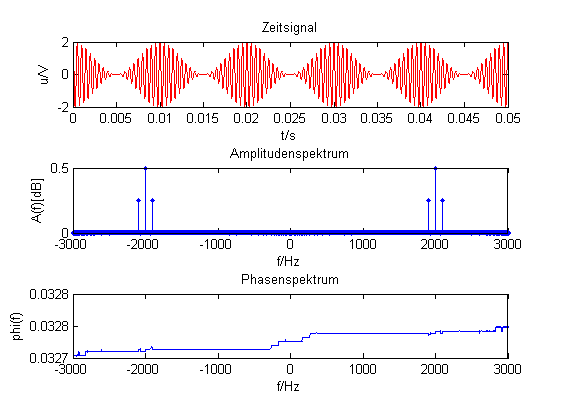
\includegraphics[scale=0.7]{Bilder/Am_Cos_2k_100Hz_mo}
                    \caption{moduliertes Signal}
                \end{figure}
        
            \end{minipage}
        
            \begin{minipage}{0.67\textwidth}
                \begin{figure}[H]
                    \label{fig:DemocosinusoT2}
                    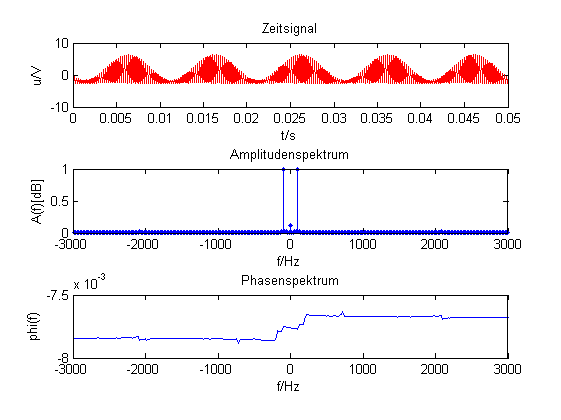
\includegraphics[scale=0.7]{Bilder/Demo_Sin_2k_100Hz_mo_ohneTiefpass}
                    \caption{demoduliertes Signal}
                \end{figure}
        
            \end{minipage}
        
        \end{tabular}
        \end{center}
        
         \begin{center}
        \begin{tabular}{ll}
        
        \hspace{-5cm}
            \begin{minipage}{0.67\textwidth}
                
                \begin{figure}[H]
                    \label{fig:DemodreieckoT}
                    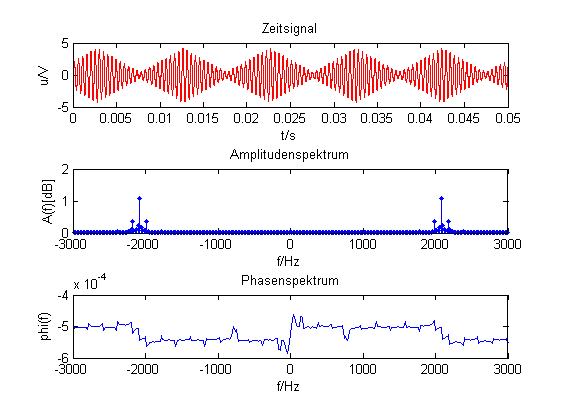
\includegraphics[scale=0.7]{Bilder/Am_Dre_2k_100Hz_mo}
                    \caption{moduliertesSignal}
                \end{figure}
        
            \end{minipage}
        
            \begin{minipage}{0.67\textwidth}
                \begin{figure}[H]
                    \label{fig:DemodreieckoT2}
                    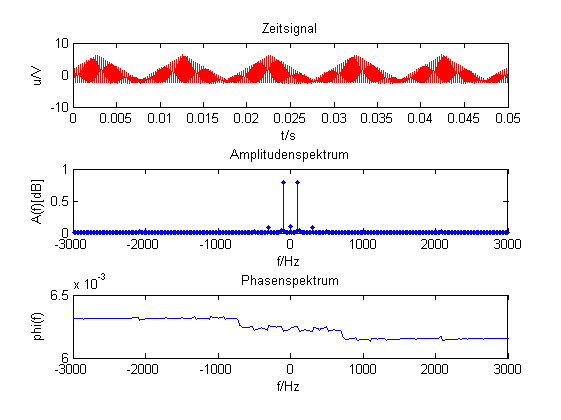
\includegraphics[scale=0.7]{Bilder/Demo_Dre_2k_100Hz_mo_ohneTiefpass}
                    \caption{demoduliertes Signal}
                \end{figure}
        
            \end{minipage}
        
        \end{tabular}
        \end{center}
        
         \begin{center}
        \begin{tabular}{ll}
        
        \hspace{-5cm}
            \begin{minipage}{0.67\textwidth}
                
                \begin{figure}[H]
                    \label{fig:DemorechteckoT}
                    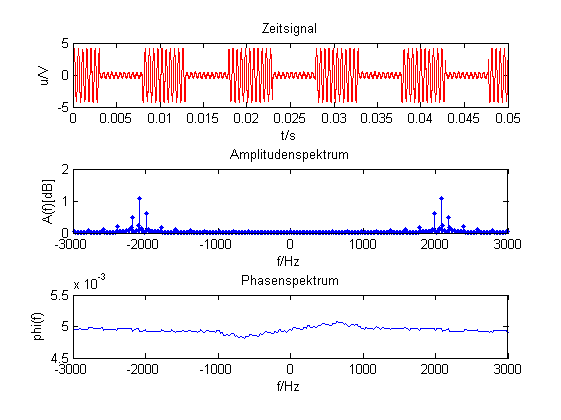
\includegraphics[scale=0.7]{Bilder/Am_Rec_2k_100Hz_mo}
                    \caption{moduliertes Signal}
                \end{figure}
        
            \end{minipage}
        
            \begin{minipage}{0.67\textwidth}
                \begin{figure}[H]
                    \label{fig:DemorechteckoT2}
                    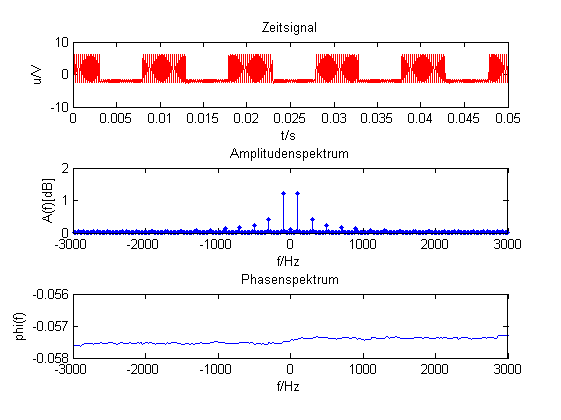
\includegraphics[scale=0.7]{Bilder/Demo_Rec_2k_100Hz_mo_ohneTiefpass}
                    \caption{demoduliertes Signal}
                \end{figure}
        
            \end{minipage}
        
        \end{tabular}
        \end{center}
               
        Zuletzt wird der Tiefpass dazu geschaltet. Was passiert, wenn man die
        Grenzfrequenz variiert und sie noch zu hoch ist, kann man in Abb.
        \ref{fig:TPmitzugrosserGF} sehen. Das Signal ähnelt dem Basisbandsignal
        schon eher, als zuvor.
        
        \begin{figure}[H]
		\begin{center}
			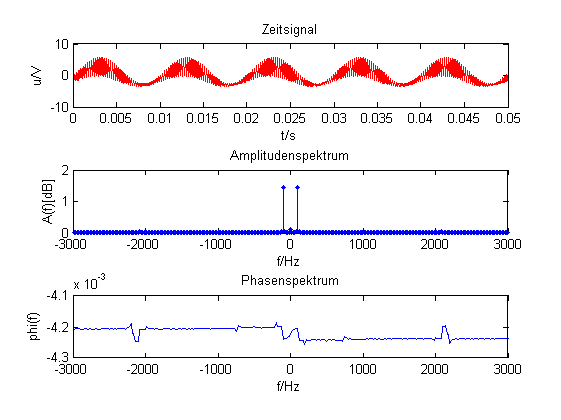
\includegraphics[width=0.8\textwidth]{Bilder/Demo_Sin_2k_100Hz_mo_mitTiefpasszugrosseGrenzfrequenz}
		\end{center}
		\caption{Demodulation mit Tiefpass mit zu großer Grenzfrequenz}
		\label{fig:TPmitzugrosserGF}
	    \end{figure}
	    
	    Mit einer niedrigeren Grenzfrequenz erhält man nahezu den Verlauf des
	    Basisbandsignals (z.B. Abb. \ref{fig:DemocosinusmT2}). Die Abweichungen
	    erklären sich dadurch, dass der Tiefpass nicht eine unendliche Steilheit besitzt und nicht alle Frequenzen
	    über 100 Herz herausfiltert.
	    
	    \begin{center}
        \begin{tabular}{ll}
        
        \hspace{-5cm}
            \begin{minipage}{0.67\textwidth}
                
                \begin{figure}[H]
                    \label{fig:DemocosinusmT}
                    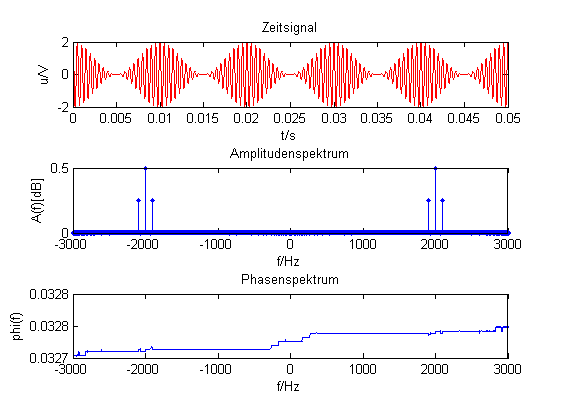
\includegraphics[scale=0.7]{Bilder/Am_Cos_2k_100Hz_mo}
                    \caption{moduliertes Signal}
                \end{figure}
        
            \end{minipage}
        
            \begin{minipage}{0.67\textwidth}
                \begin{figure}[H]
                    \label{fig:DemocosinusmT2}
                    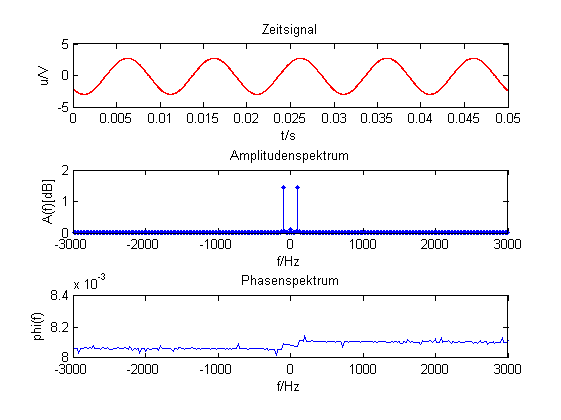
\includegraphics[scale=0.7]{Bilder/Demo_Sin_2k_100Hz_mo_mitTiefpass}
                    \caption{demoduliertes Signal}
                \end{figure}
        
            \end{minipage}
        
        \end{tabular}
        \end{center}
        
        \begin{center}
        \begin{tabular}{ll}
        
        \hspace{-5cm}
            \begin{minipage}{0.67\textwidth}
                
                \begin{figure}[H]
                    \label{fig:DemodreieckmT}
                    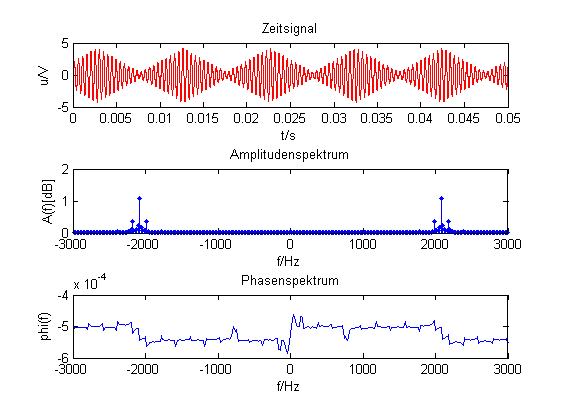
\includegraphics[scale=0.7]{Bilder/Am_Dre_2k_100Hz_mo}
                    \caption{moduliertes Signal}
                \end{figure}
        
            \end{minipage}
        
            \begin{minipage}{0.67\textwidth}
                \begin{figure}[H]
                    \label{fig:DemodreieckmT2}
                    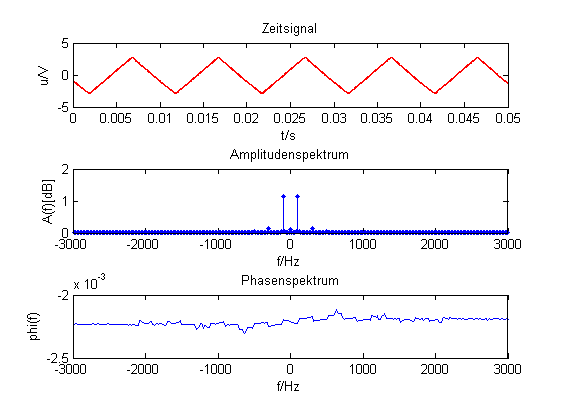
\includegraphics[scale=0.7]{Bilder/Demo_Dre_2k_100Hz_mo_mitTiefpass}
                    \caption{demoduliertes Signal}
                \end{figure}
        
            \end{minipage}
        
        \end{tabular}
        \end{center}
        
        \begin{center}
        \begin{tabular}{ll}
        
        \hspace{-5cm}
            \begin{minipage}{0.67\textwidth}
                
                \begin{figure}[H]
                    \label{fig:DemodreieckmT}
                    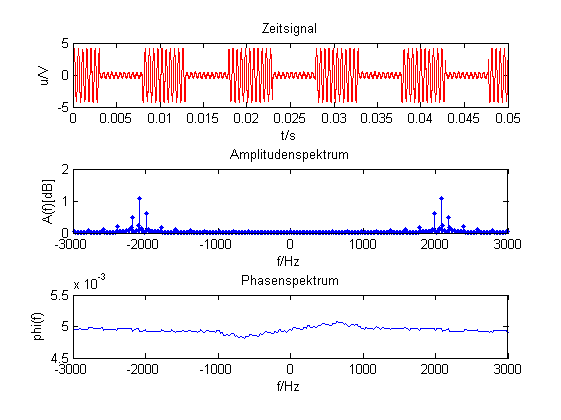
\includegraphics[scale=0.7]{Bilder/Am_Rec_2k_100Hz_mo}
                    \caption{moduliertes Signal}
                \end{figure}
        
            \end{minipage}
        
            \begin{minipage}{0.67\textwidth}
                \begin{figure}[H]
                    \label{fig:DemodreieckmT2}
                    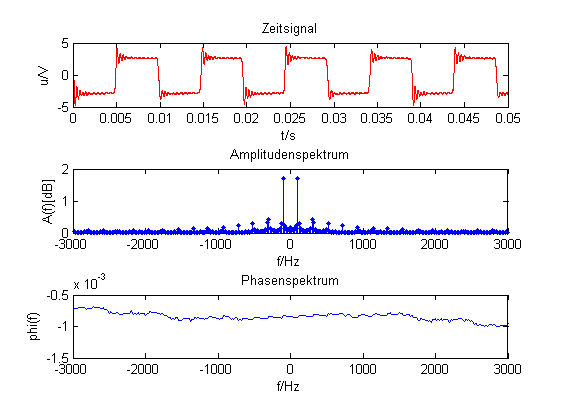
\includegraphics[scale=0.7]{Bilder/Demo_Rec_2k_100Hz_mo_mitTiefpass}
                    \caption{demoduliertes Signal}
                \end{figure}
        
            \end{minipage}
        
        \end{tabular}
        \end{center}
        
    \end{quote}
    
\end{quote}


\section{FM}
\begin{quote}
    
    
    \subsection{Labordurchführung}
    \begin{quote}
    
        Die Frequenzmodulation wird mit Hilfe des VCO-Moduls auf dem ETT 101 durchgeführt. Dabei wird ein 3 kHz Sinussignal mit
        der Amplitude 1 Volt aus dem Frequenzgenerator auf den VCO Input gelegt, der FREQ-Controller auf die mittlere Position
        gestellt, der Schalter auf Lo gestellt (Frequenzbereich von 1 bis 15 kHz) und das Gain auf zwei Drittel des Maximalwerts
        gestellt.
        Von diesem Signal sollte das Spektrum mit dem Picoscope aufgenommen werden und $K_{FM}$ und $\Delta f_{max}$ anhand der
        Verläufe von Nutz- und Trägersignal bestimmt werden.\\
        
        Dabei sollen die Auswirkungen einer Variation des Nutzsignals in der Frequenz und der Amplitude untersucht werden. Für die
        Amplitude wird nach dem Parsevalschen Theorem erwartet, dass sich die Amplituden im Zeit- und Frequenzbereich proportional
        verhält.\\
        Außerdem werden nach Fouriere für eine höhere Nutzfrequenz mehr Frequenzen benötigt um per Überlagerung das modulierte
        Signal zu erstellen. Auch bei Höheren Amplituden werden mehr Frequenzen benötigt, da das Trägersignal mehr gestaucht
        wird\\
        \\
        Zur FM-Demodulation haben wir im Praktikum die FM-PFM-Umwandlung genutzt, da es ein relativ einfaches Verfahren ist.
        Hierbei wird das Signal zunächst durch einen Komparator in eine polare Rechteckfolge umgewandelt.
        Als Referenz für den Comparator wird \si{0}{\volt} eingestellt, damit jede positive Halbwelle des modulierten Signals zu
        einem positiven Rechteck wird und jede negative zu \si{0}{\volt} (siehe Abb.
        \ref{fig:fct Com}).\\
        Das modulierte Signal hat Bereiche in denen die Frequenz höher ist, dass heißt die Nulldurchgänge häufiger und Bereiche in
        denen die Frequenz niedrieger ist, dass heißt die Nulldurchgänge seltener sind. Bei der Demodulation wird dies ausgenutzt,
        indem ein Komparator wie oben beschrieben bei jedem positiven Signalverlauf eine  eins ausgibt und bei negativem
        Signalverlauf eine null. Dabei variiert die breite der Rechteckt mit der Frequenz. Nach dem Komperator gibt der Twin Pulse
        Generator bei jeder steigender Flanke ein Puls fester breite aus, dass heißt die Pulse haben im Anschluss unterschiedliche
        Abstände.\\
        Anschließend wird das Signal noch durch einen Twin Pulse Generator geführt, der aus jeder steigenden Flanke einen
        Deltaimpuls macht bzw. in Realität ein Rechteckimpuls mit fester Breite.
        Aellerdings variieren die Abstände der Pulse in Abhängigkeit der Frequenz.Die Regler Width und Delay, die für die Breite
        der Rechteckimpulse und die Verzögerung zwischen den beiden Rechteckimpulsen steht, damit das Rechteck möglichst nahe an
        einen Deltaimpuls heran kommt und, damit der Puls auf dem Ausgang Q2, den wir ausschließlich benutzen, mit möglichst wenig
        Verzögerung ausgegeben wird.\\
        Zuletzt wird das Signal noch tiefpass-gefiltert, um aus der Häufigkeit der Pulse wieder das Analoge ausgangssignal zu
        machen.
        
      \end{quote}
     
    \subsection{Auswertung}
    \begin{quote}
        
        \subsubsection{Trägerfrequenz $f_c$ \& Proportionalitätskonstante $K_{FM}$}
            
            
            
            \begin{center}
            \begin{tabular}{ll}
            
            \hspace{-4cm}
                \begin{minipage}{0.67\textwidth}
                    
                    \begin{figure}[H]
                        \label{fig:Tmax}
                        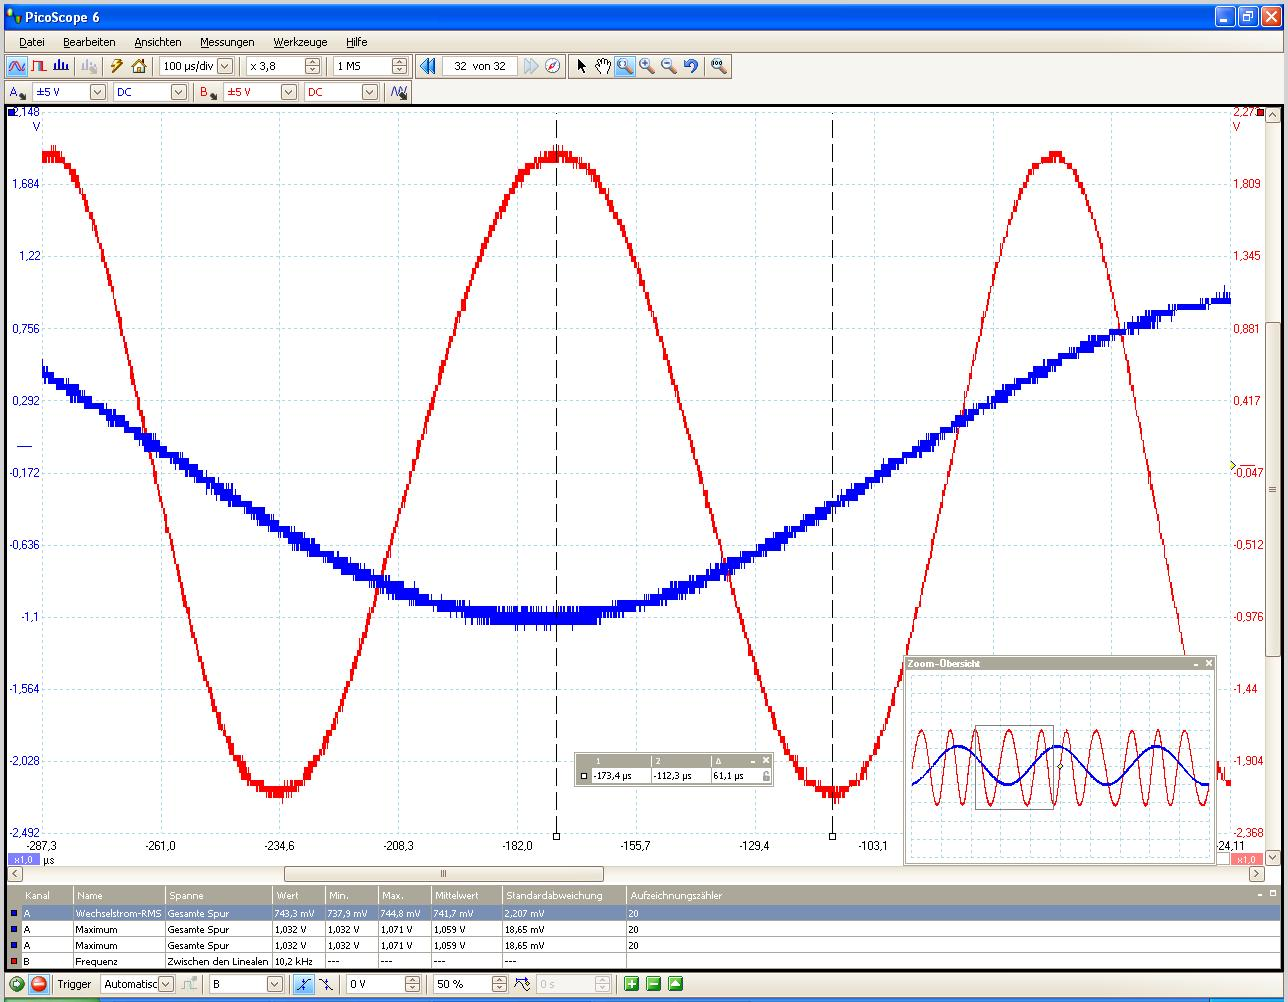
\includegraphics[scale=0.25, trim = 0mm 0mm 0mm 0mm, clip]{Bilder/Tmax}
                        \caption{Tmax = $61,1 \mu s$}
                    \end{figure}
                    
                \end{minipage}
                
                \begin{minipage}{0.67\textwidth}
                    \begin{figure}[H]
                        \label{fig:Tmin}
                        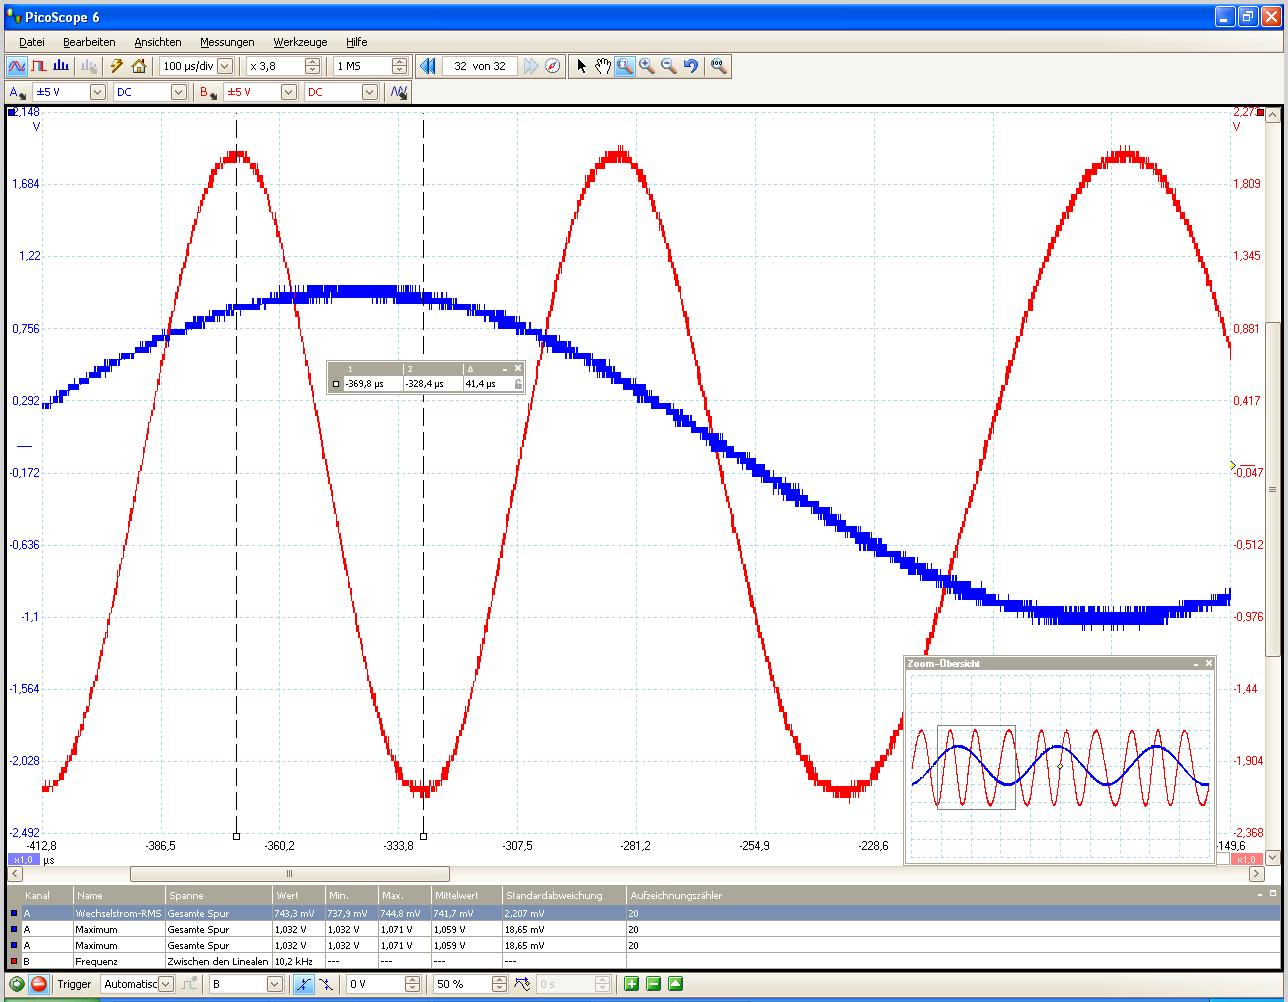
\includegraphics[scale=0.25, trim = 0mm 0mm 0mm 0mm, clip]{Bilder/Tmin}
                        \caption{Tmin = $41,4 \mu s$}
                    \end{figure}
                    
                \end{minipage}
            
            \end{tabular}
            \end{center}
            \vspace{2em}
            
        \begin{quote}
                
            Auf $K_{FM}$ kann man, bei bekannter Eingangsamplitude, mit der minimalen und maximalen Frequenz des modulierten
            Signals zurückschließen. Der Faktor $K_{FM}$ ist laut der FM-Modulationsformel \ref{equ:fm} proportional zur
            min-/maximalen Frequenz des Modulierten Signals bei min-/maximaler Amplitude des Nutzsignals.
            
            
            \begin{equation*}
            \begin{split}
            \\
                \Delta f_{max} &\approx \frac{1}{2} (\frac{1}{T_{min}} - \frac{1}{T_{max}})\\
                               &= \frac{1}{2} (\frac{1}{4\cdot41,4 \mu s}
                               -\frac{1}{4\cdot61,1 \mu s})\\
                               &= 973,4972 \frac{1}{s}\\
            \\
                K_{FM} &=\frac{2 \pi \Delta f_{max}}{A_u}\\
                       &= \frac{2 \pi \p 3894 \frac{1}{s}}{1V}\\
                       &=   6116 \frac{1}{Vs}
            \\
            \end{split}
            \end{equation*}
            \label{equ:}
            
            Die Trägerfrequenz von \si{10}{kHz} lässt dich sehr gut an dem Folgenden Spektrum \ref{fig:freq_1k} (roter Plot)
            eines modulierten \si{1}{kHz} Sinus-Signals (blauer Plot) erkennen. Hier befindet sich die Mitte des Spektrums exakt bei
            \si{10}{kHz} woran sich die Trägerfrequenz ablesen lässt, da das Nutzsignal (der Sinus) das frequenzspektrum
            gleichmäßig nach rechts und links ausdehnt.
            
            \begin{figure}[H]
            \centering
                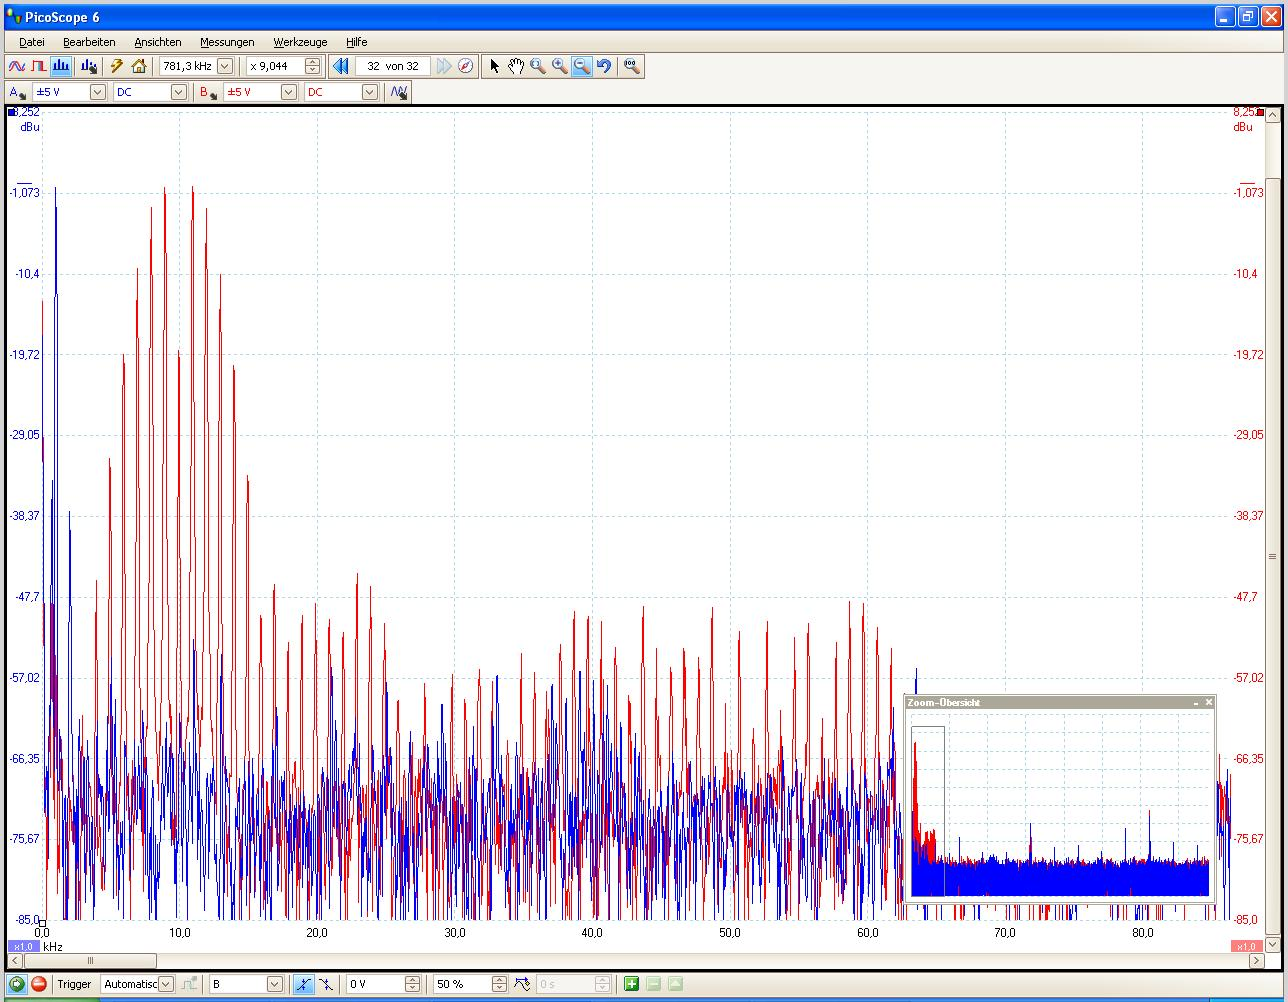
\includegraphics[scale=0.5, trim = 0.25cm 1.3cm 1cm 3.2cm, clip]{Bilder/freq_1k}
                    \caption{Frequenzmoduliertes 1kHz Signal}
                    \label{fig:freq_1k}
            \end{figure}
            
            
        \end{quote}
        
        \subsubsection{Auswirkung der Amplitude des Sendesignals auf das Ausgangssignal}
        \begin{quote}
            
            \begin{center}
            \begin{tabular}{ll}
            
            \hspace{-5cm}
                \begin{minipage}{0.6\textwidth}
                    \begin{figure}[H]
                        \label{fig:f100_05}
                        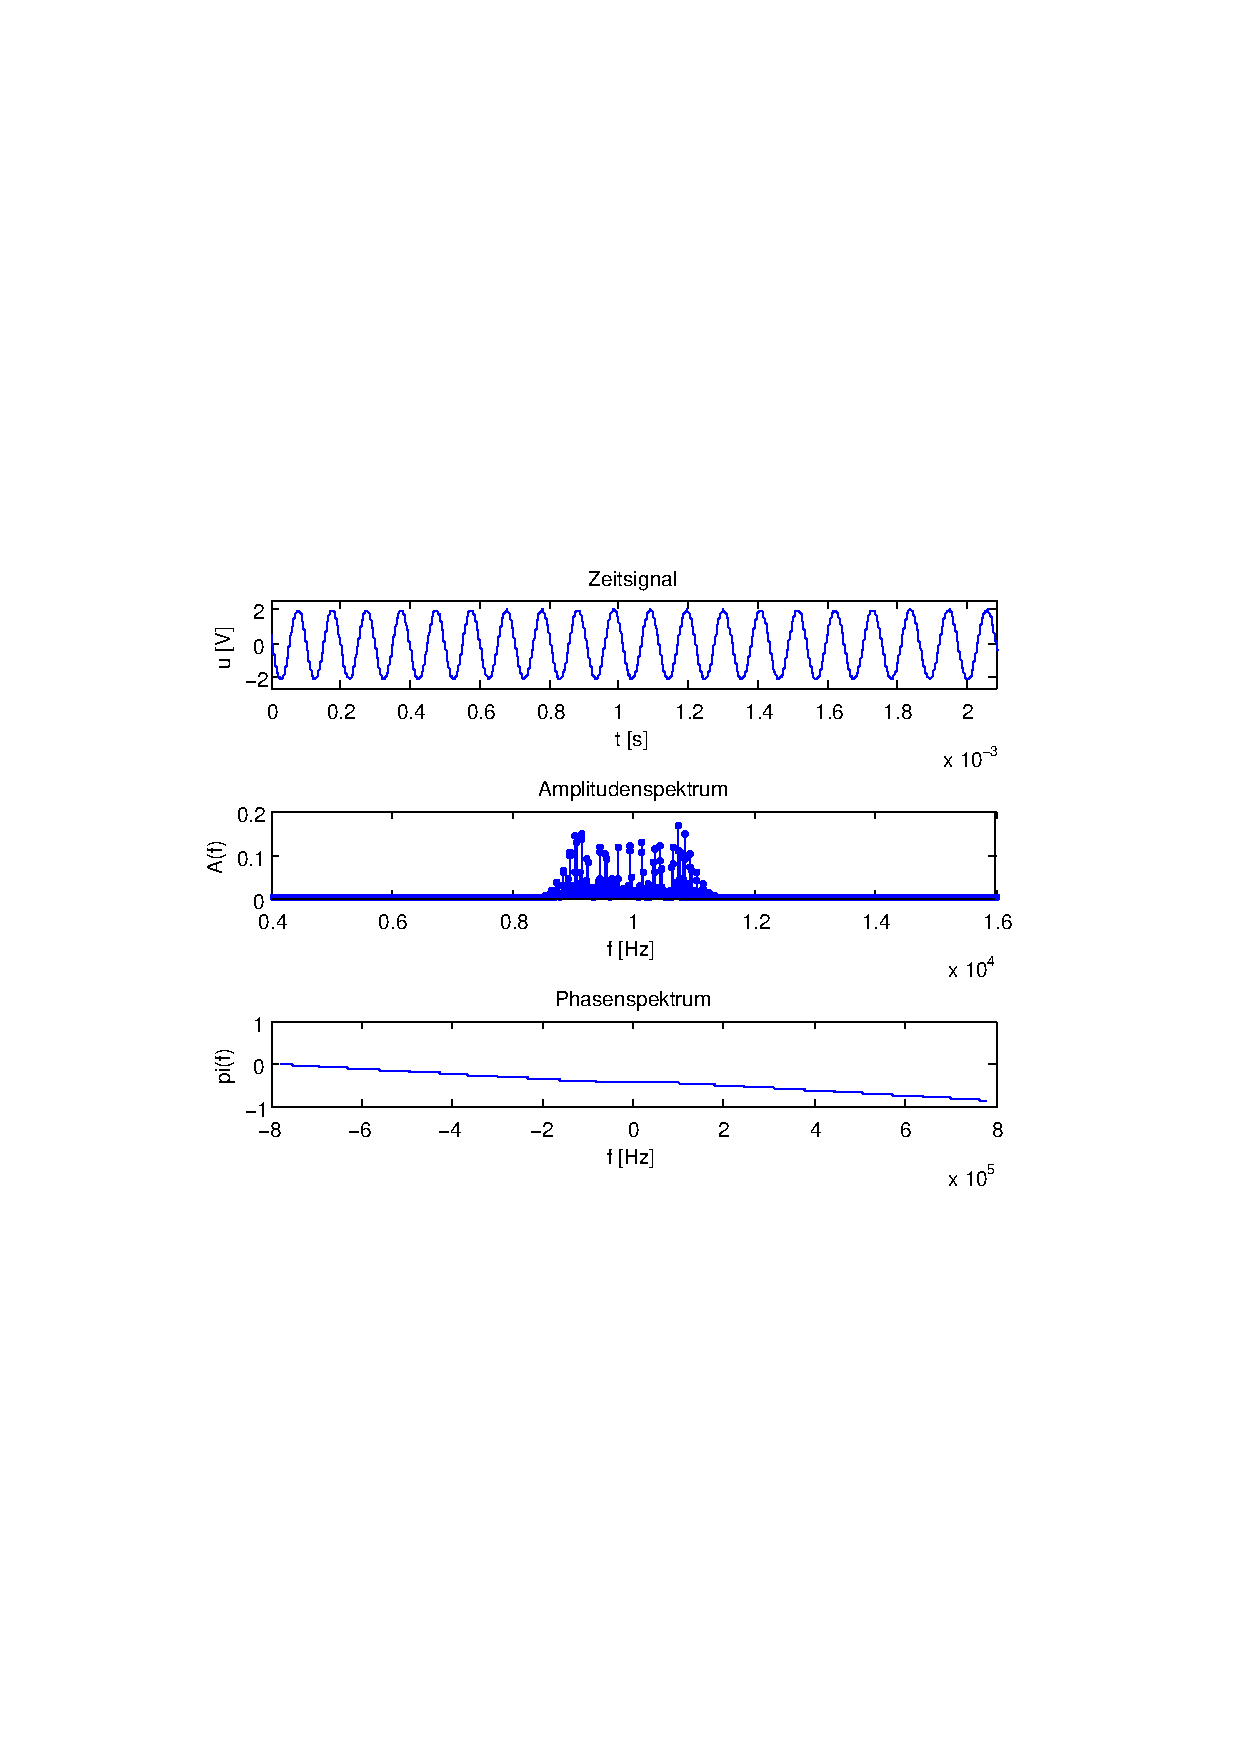
\includegraphics[scale=0.7, trim = 35mm 100mm 35mm 95mm, clip]{Bilder/f100_05}
                        \caption{FM von \SI{100}{\hertz} mit \SI{0,5}{\volt} Amplitude}
                    \end{figure}
                \end{minipage}
                
                \begin{minipage}{0.6\textwidth}
                    \begin{figure}[H]
                        \label{fig:f100_1}
                        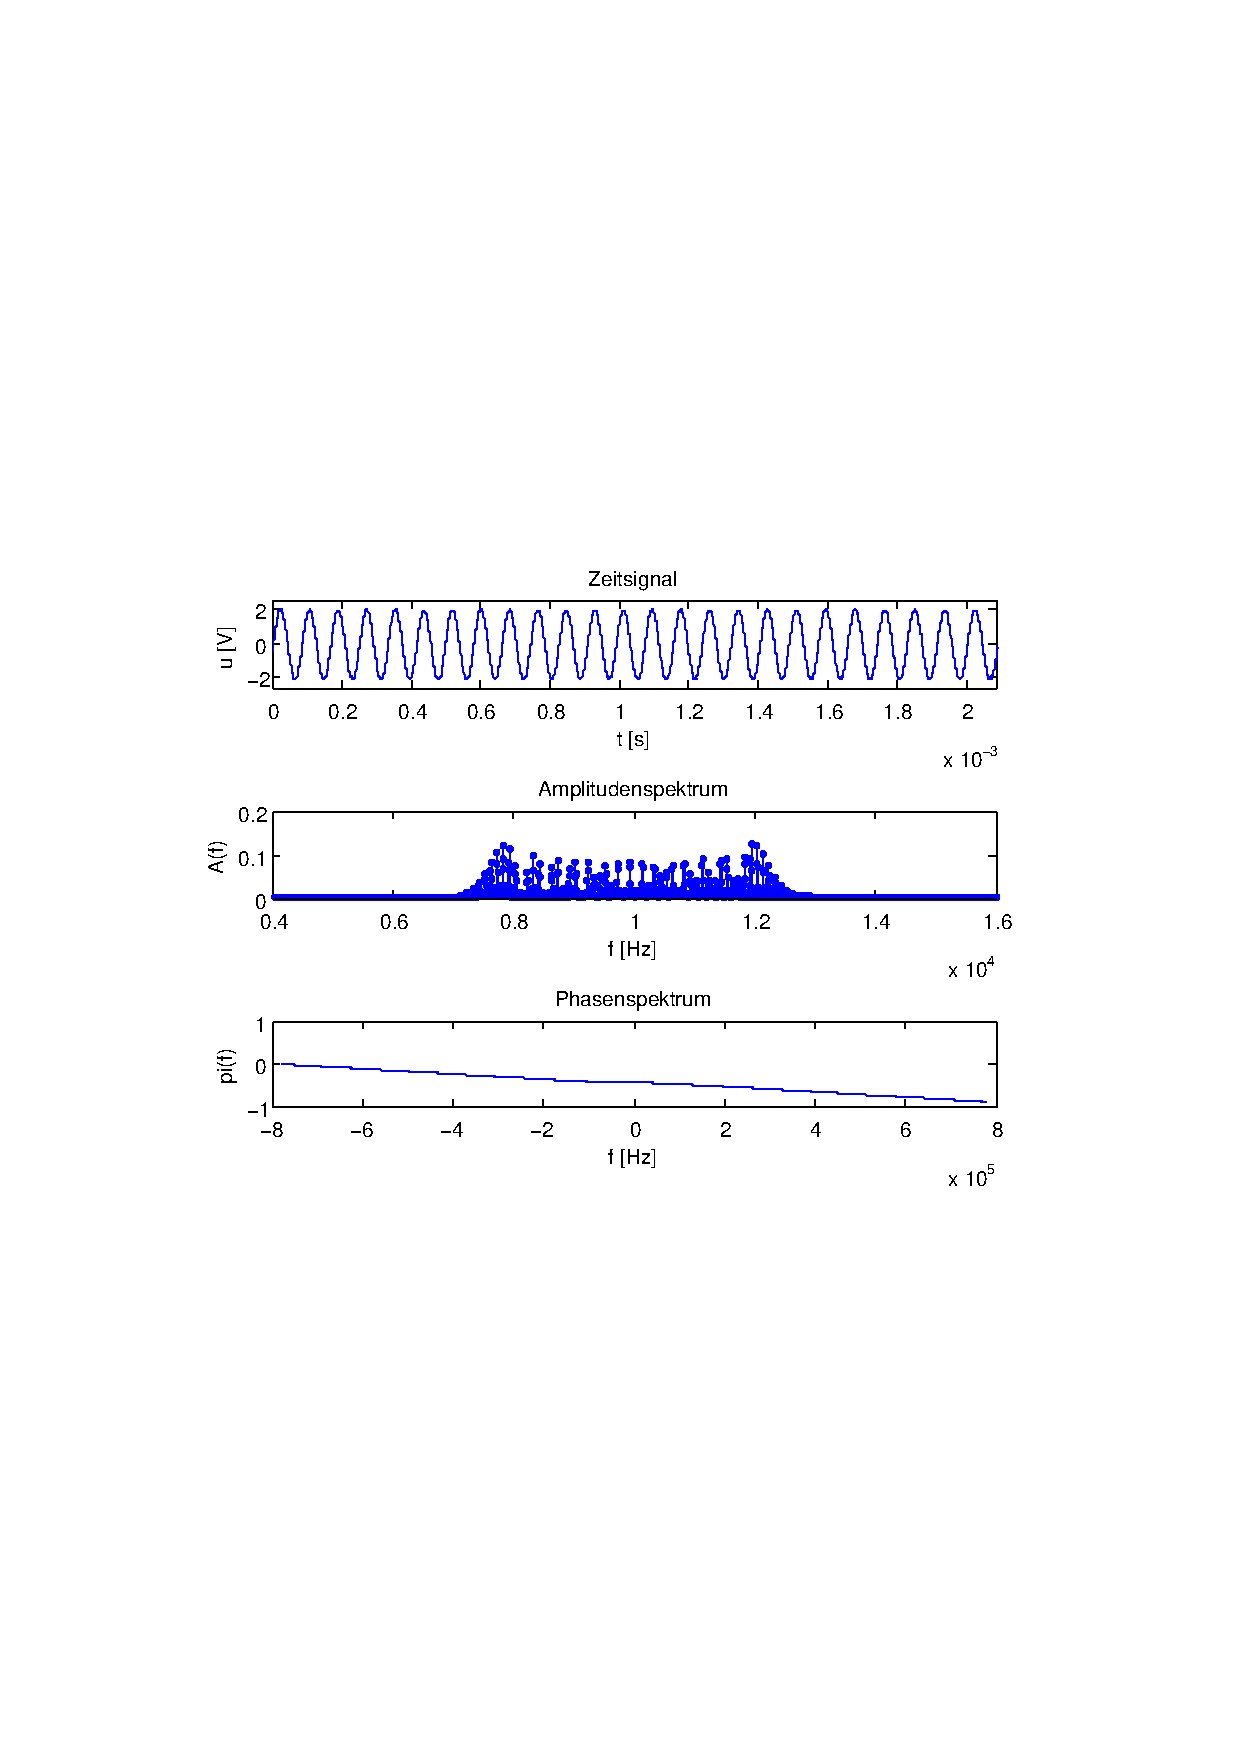
\includegraphics[scale=0.7, trim = 35mm 100mm 35mm 95mm, clip]{Bilder/f100_1}
                        \caption{FM von \SI{100}{\hertz} mit \SI{1}{\volt} Amplitude}
                    \end{figure}
                \end{minipage}
            
            \end{tabular}
            \end{center}
            
            \begin{figure}[H]
            \centering
                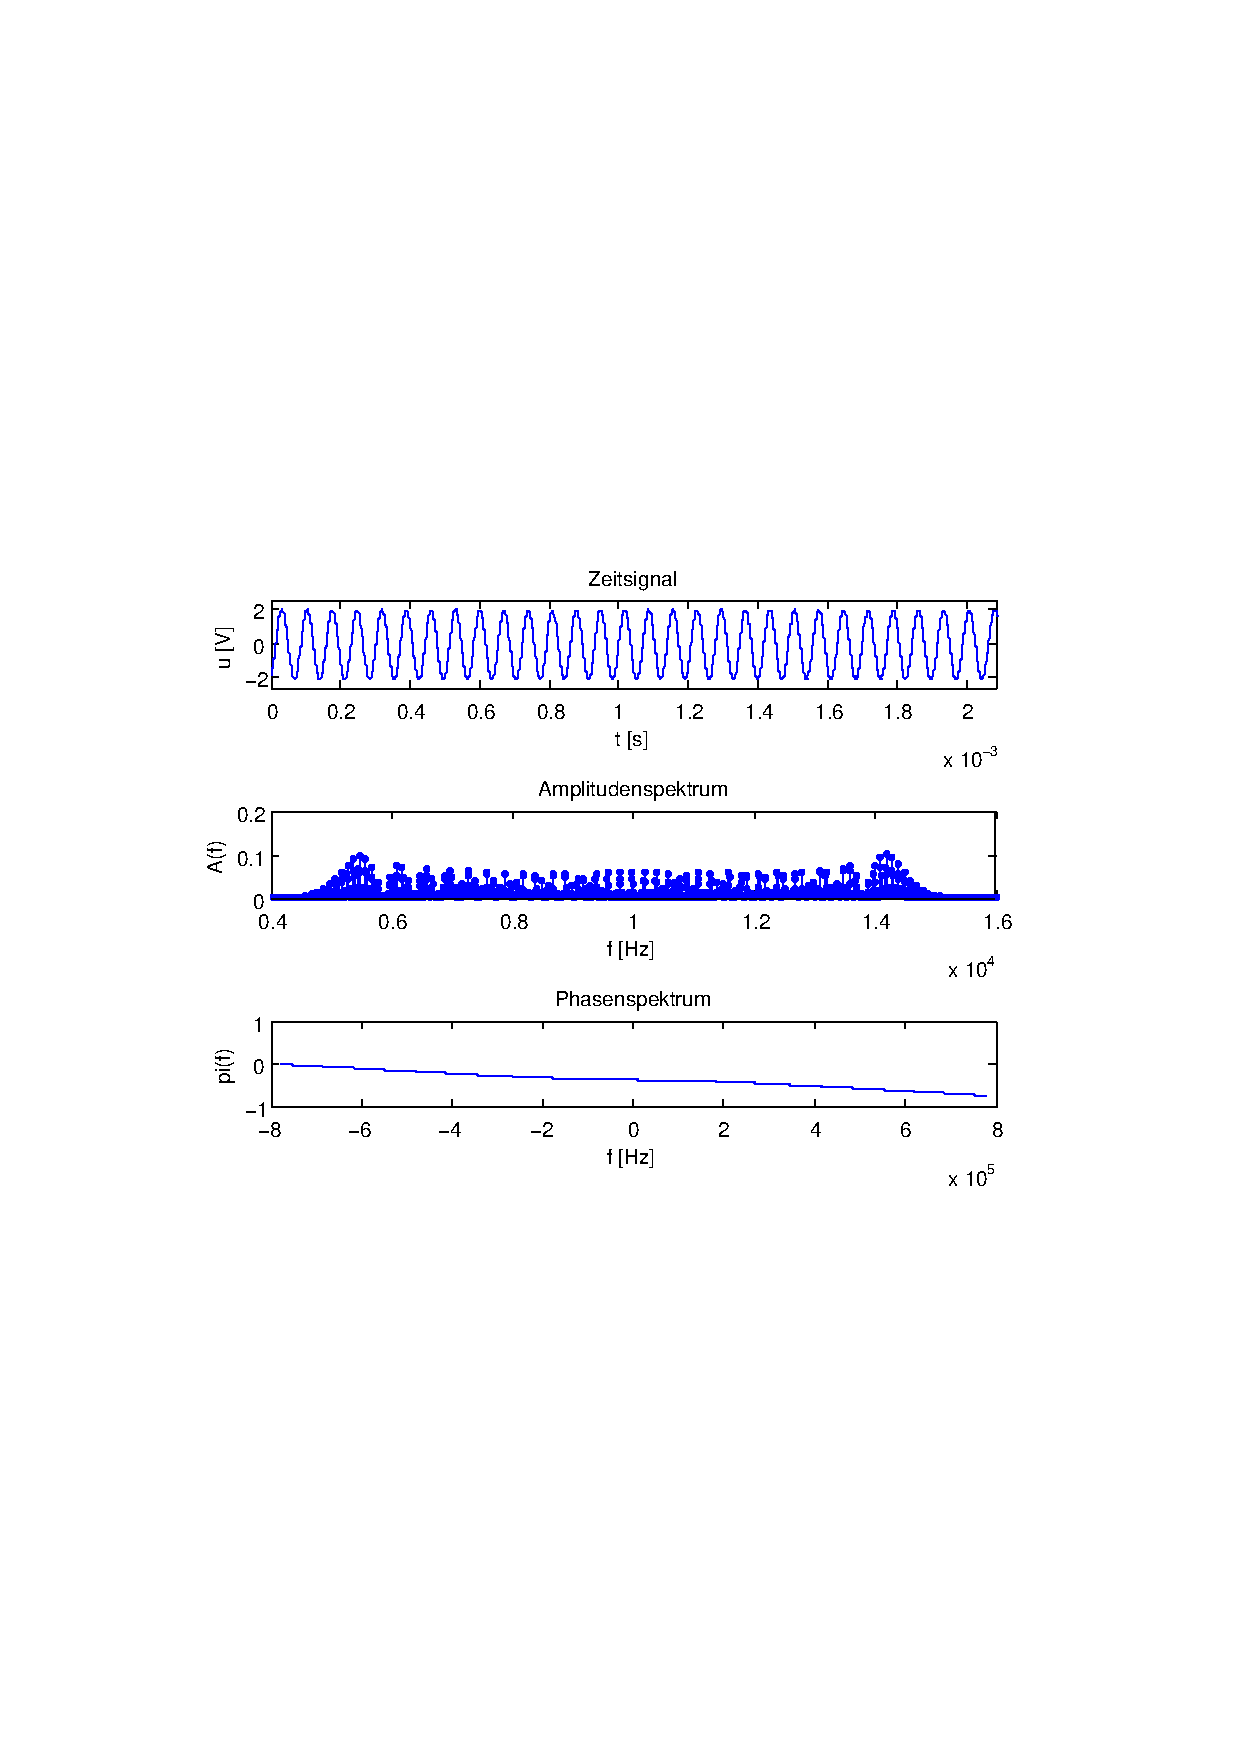
\includegraphics[scale=0.7, trim = 35mm 100mm 35mm 95mm, clip]{Bilder/f100_2}
                    \caption{FM von \SI{100}{\hertz} mit \SI{2}{\volt} Amplitude}
                    \label{fig:f100_2}
            \end{figure}
            
            
            
        \end{quote}

        \subsubsection{Auswirkung der Frequenz des Sendesignals auf das Ausgangssignal}
        \begin{quote}
            
            
            
            \begin{center}
            \begin{tabular}{ll}
            
            \hspace{-5cm}
                \begin{minipage}{0.6\textwidth}
                    \begin{figure}[H]
                        \label{fig:f100_05}
                        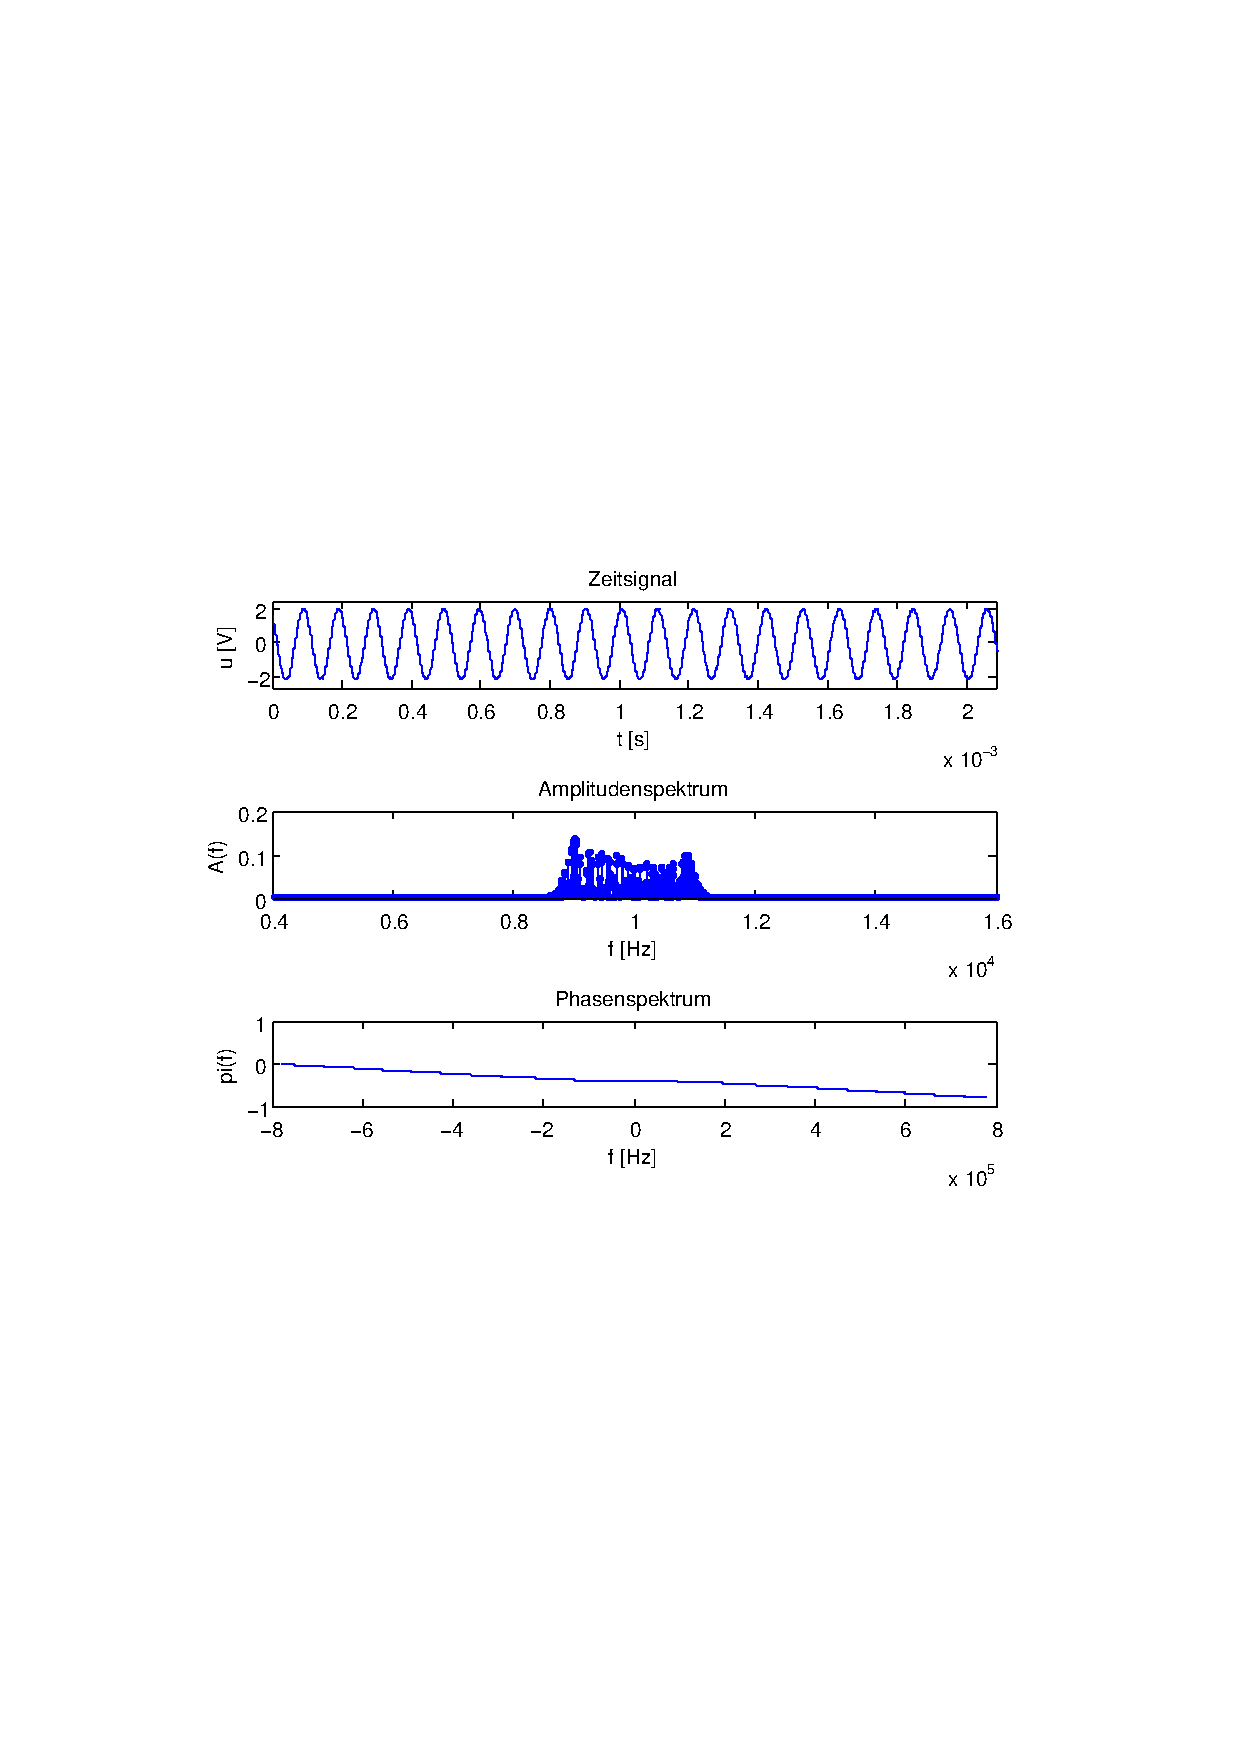
\includegraphics[scale=0.7, trim = 35mm 100mm 35mm 95mm, clip]{Bilder/f50_05}
                        \caption{FM von \SI{500}{\hertz} mit \SI{0,5}{\volt} Amplitude}
                    \end{figure}
                \end{minipage}
                
                \begin{minipage}{0.6\textwidth}
                    \begin{figure}[H]
                        \label{fig:f100_1}
                        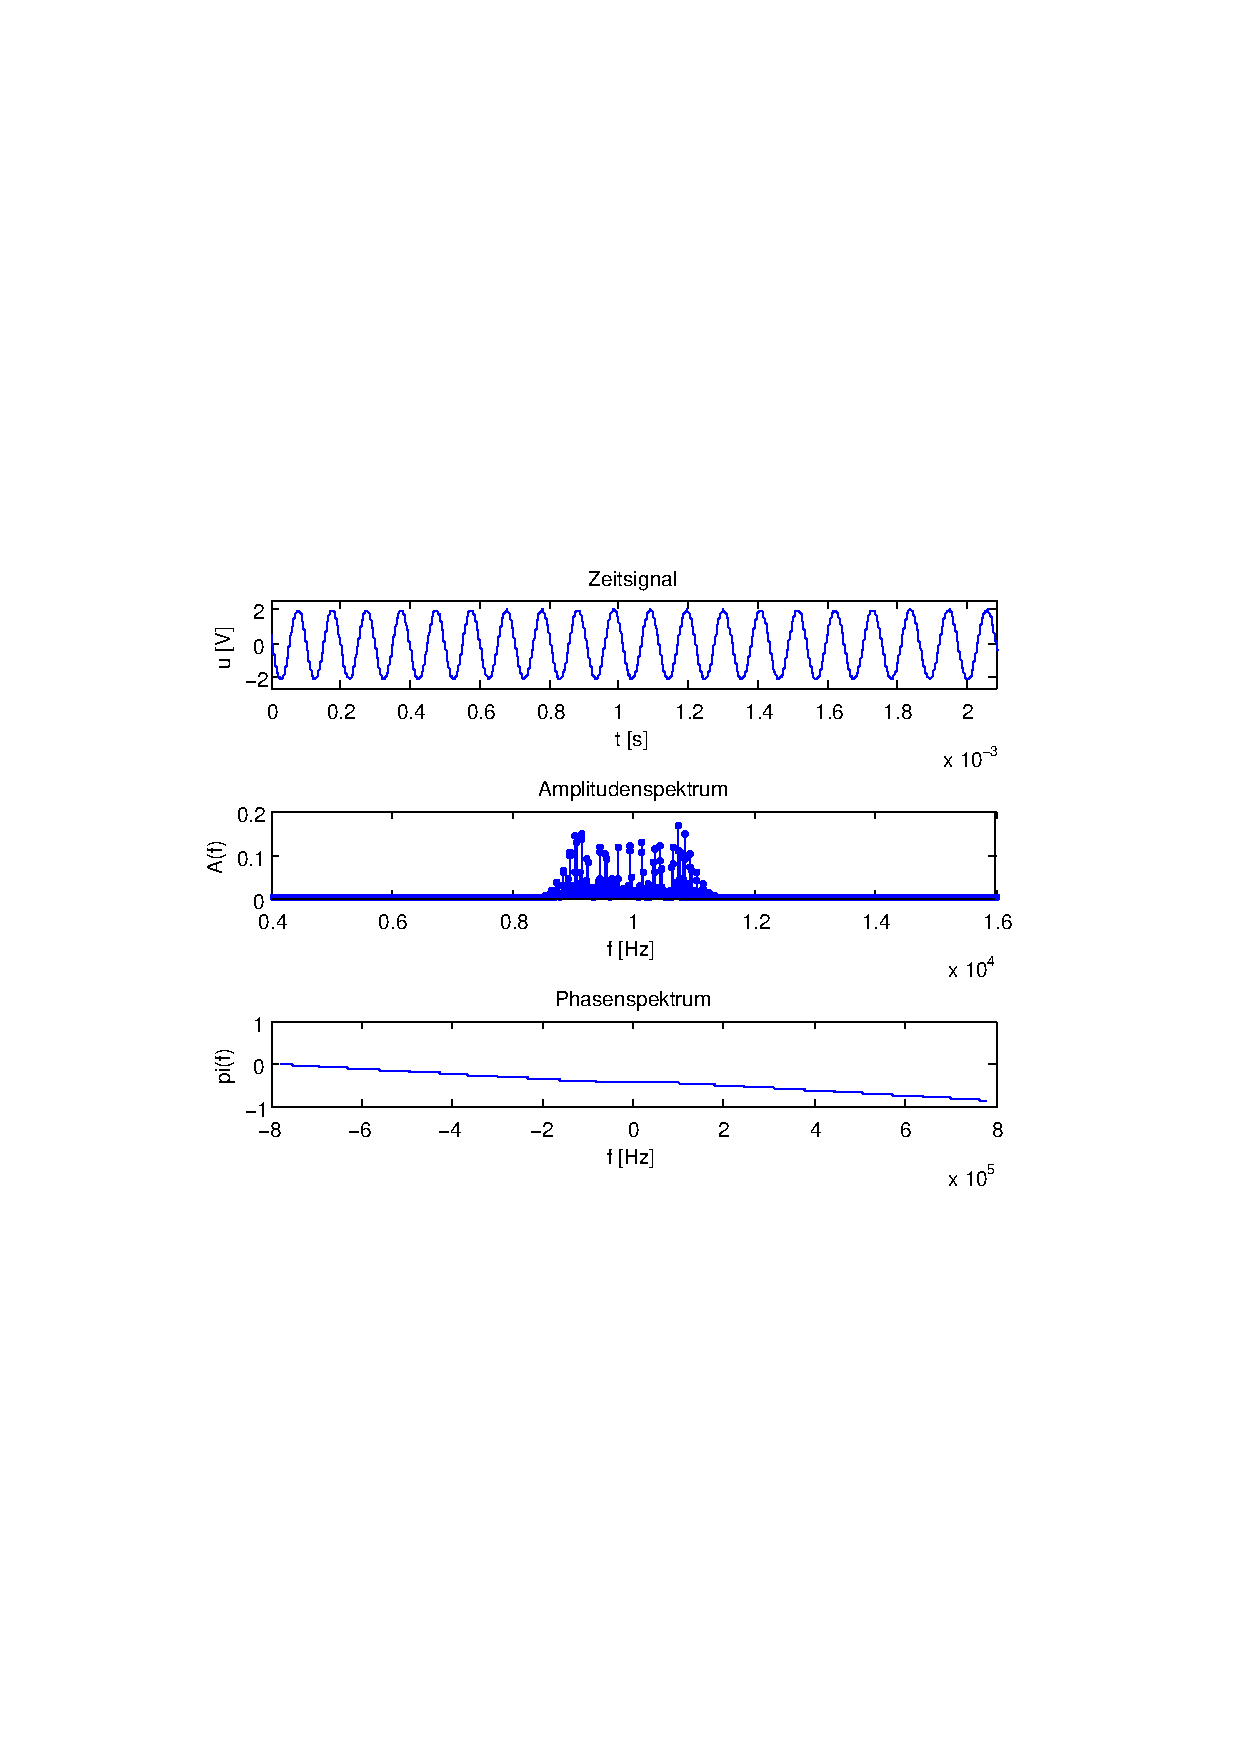
\includegraphics[scale=0.7, trim = 35mm 100mm 35mm 95mm, clip]{Bilder/f100_05}
                        \caption{FM von \SI{100}{\hertz} mit \SI{0,5}{\volt} Amplitude}
                    \end{figure}
                \end{minipage}
            
            \end{tabular}
            \end{center}
            
            \begin{figure}[H]
            \centering
                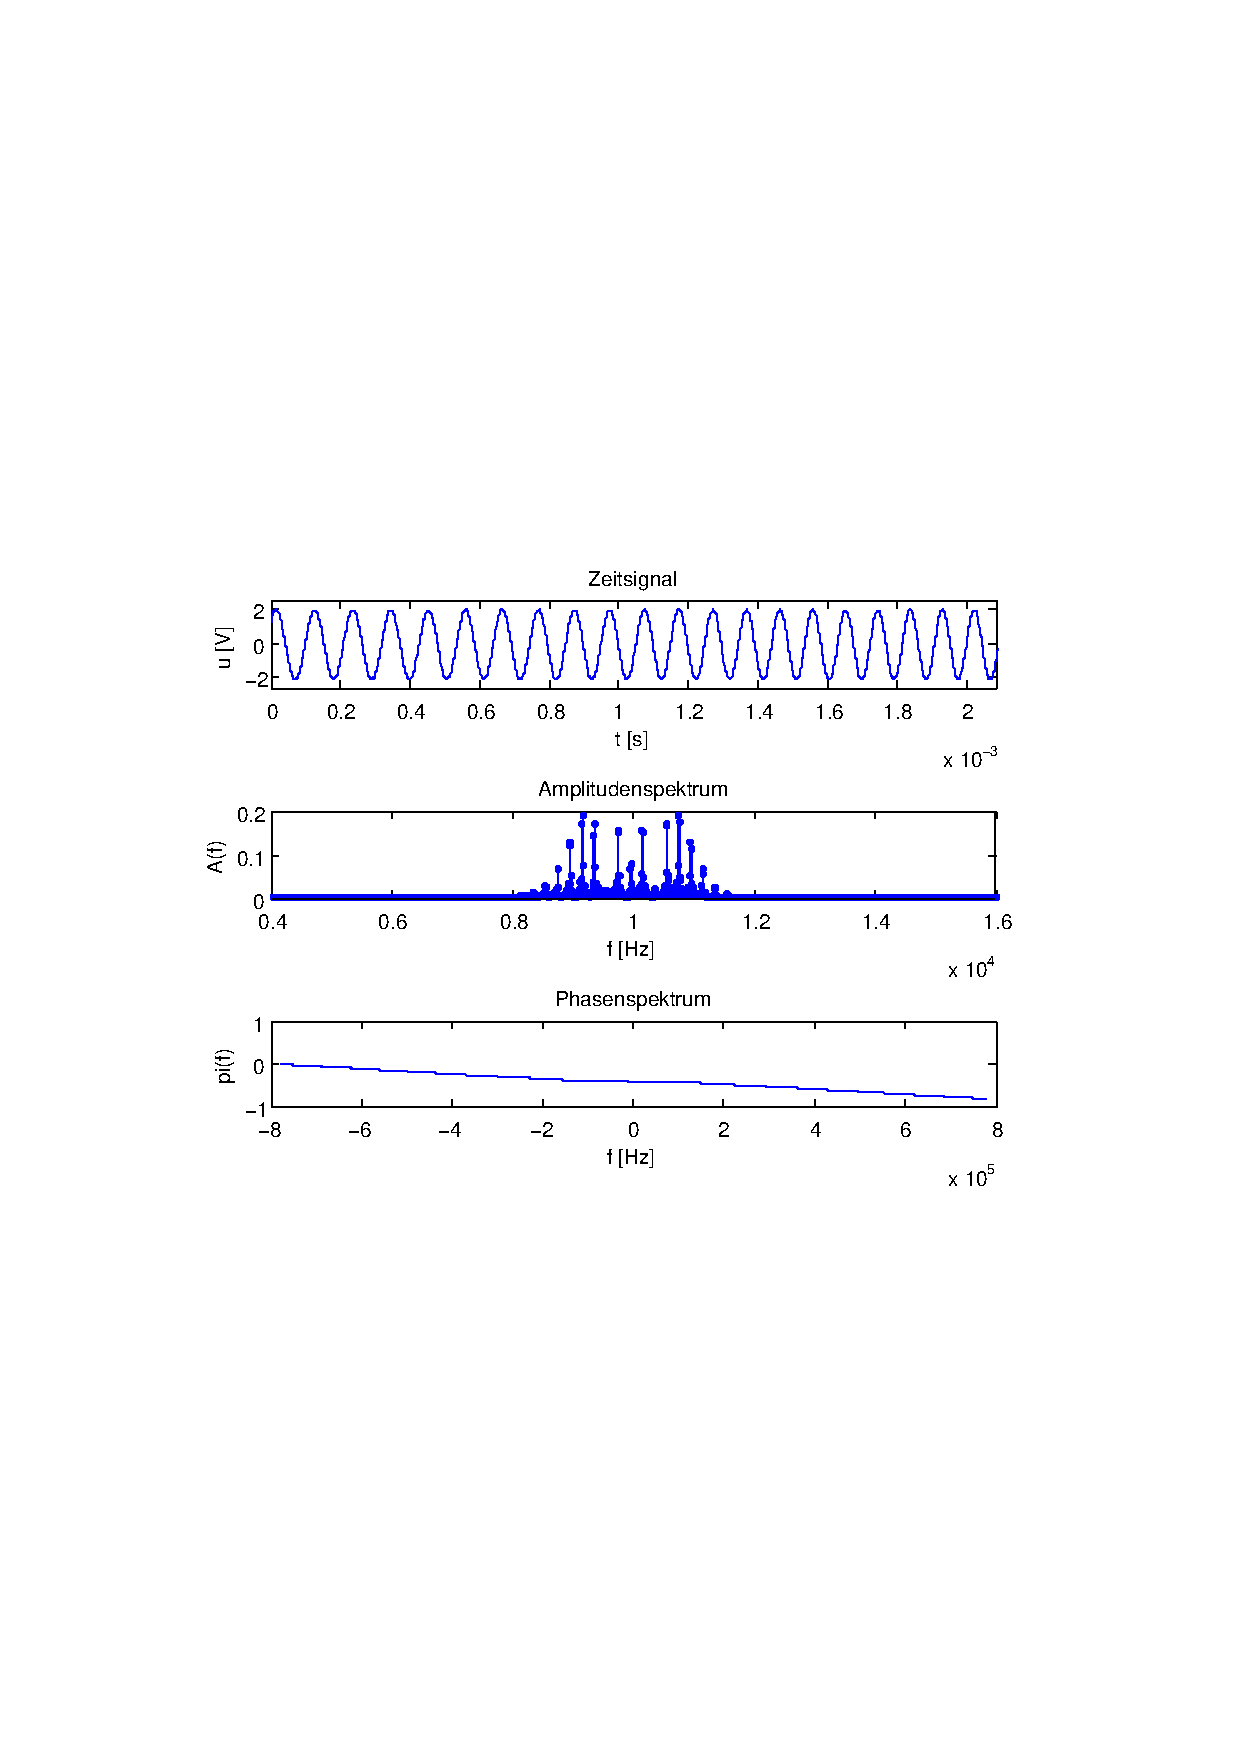
\includegraphics[scale=0.7, trim = 35mm 100mm 35mm 95mm, clip]{Bilder/f200_05}
                    \caption{FM von \SI{200}{\hertz} mit \SI{0,5}{\volt} Amplitude}
                    \label{fig:f100_2}
            \end{figure}
            
        \end{quote}

        
        
        \subsubsection{Auswirkung der Frequenz und der Amplitude des Sendesignals auf das Ausgangssignal}
        \begin{quote}
            
            
            \begin{center}
            \begin{tabular}{ll}
            
            \hspace{-5cm}
                \begin{minipage}{0.6\textwidth}
                    \begin{figure}[H]
                        \label{fig:f100_05}
                        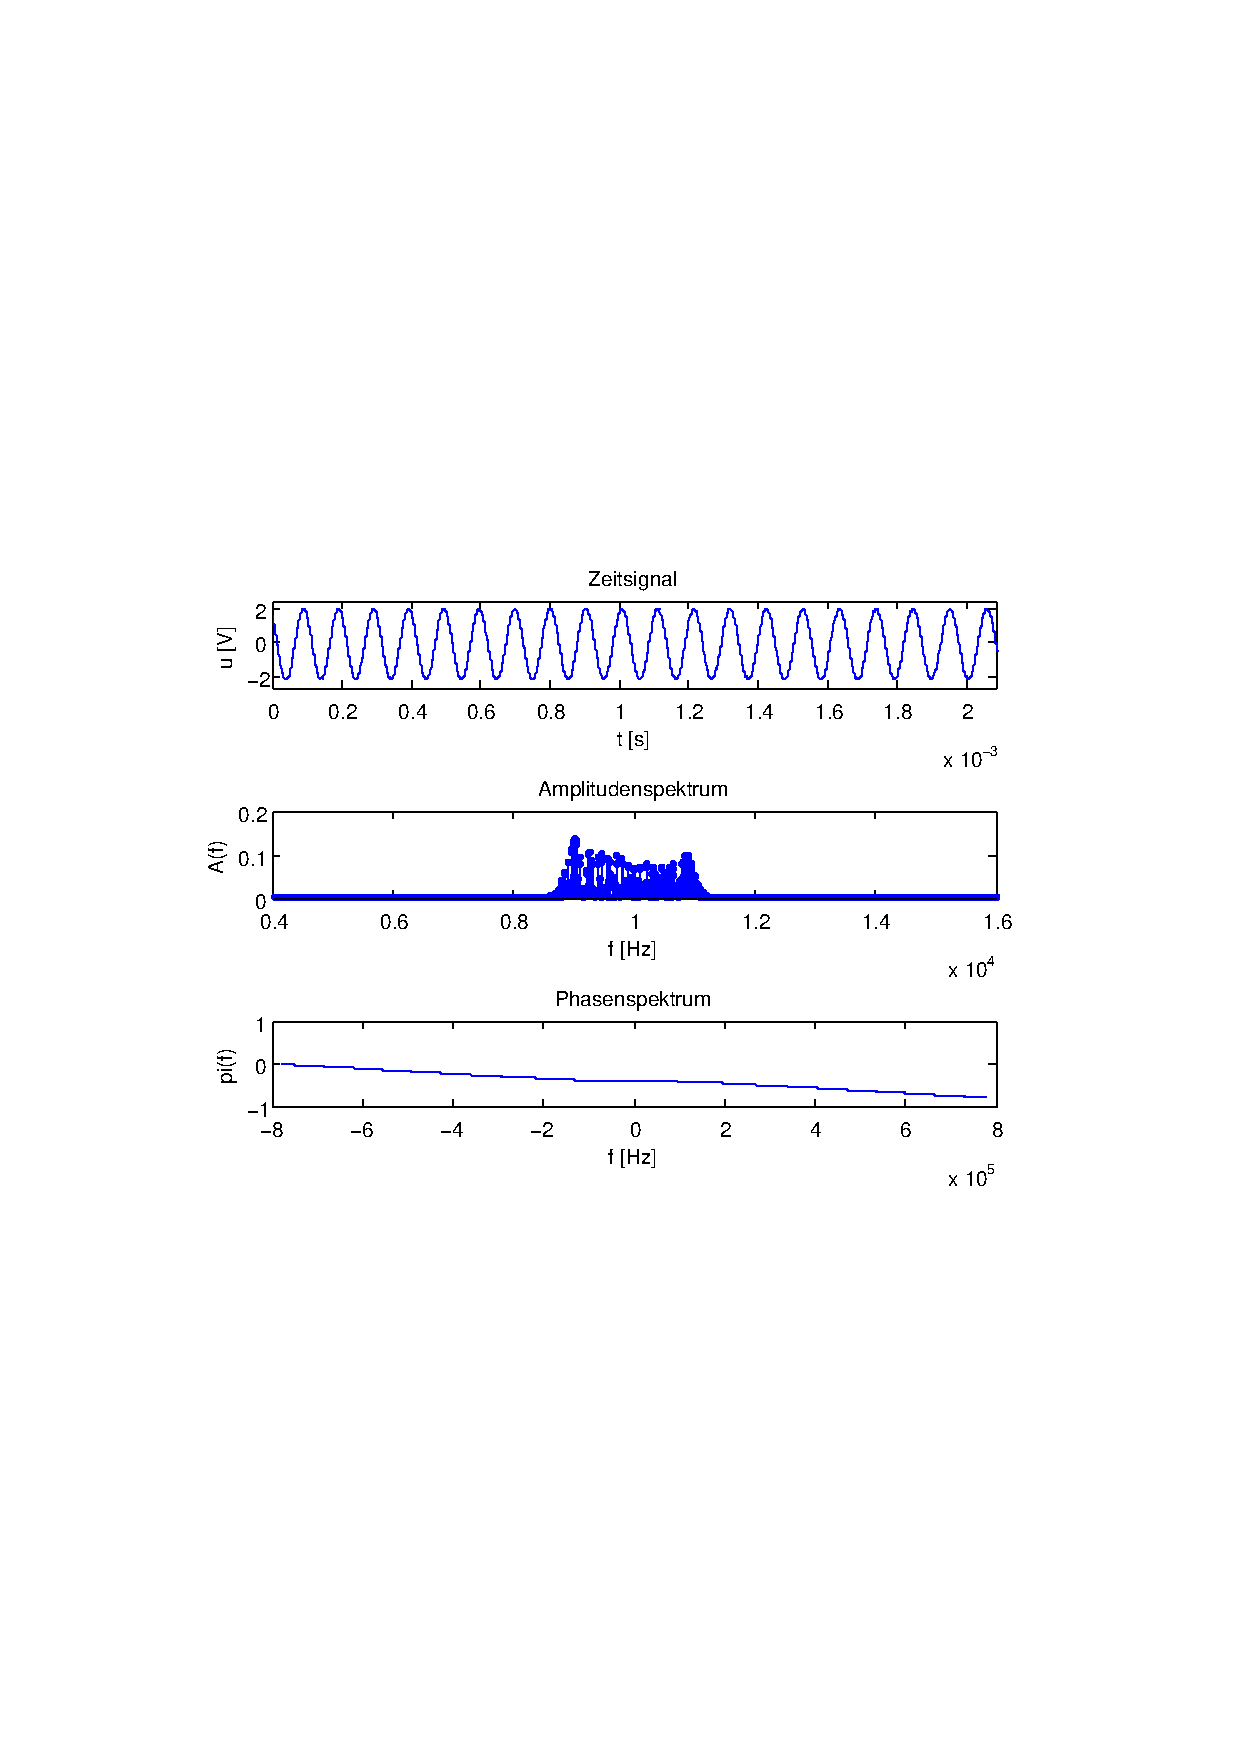
\includegraphics[scale=0.7, trim = 35mm 100mm 35mm 95mm, clip]{Bilder/f50_05}
                        \caption{FM von \SI{50}{\hertz} mit \SI{0,5}{\volt} Amplitude}
                    \end{figure}
                \end{minipage}
                
                \begin{minipage}{0.6\textwidth}
                    \begin{figure}[H]
                        \label{fig:f100_1}
                        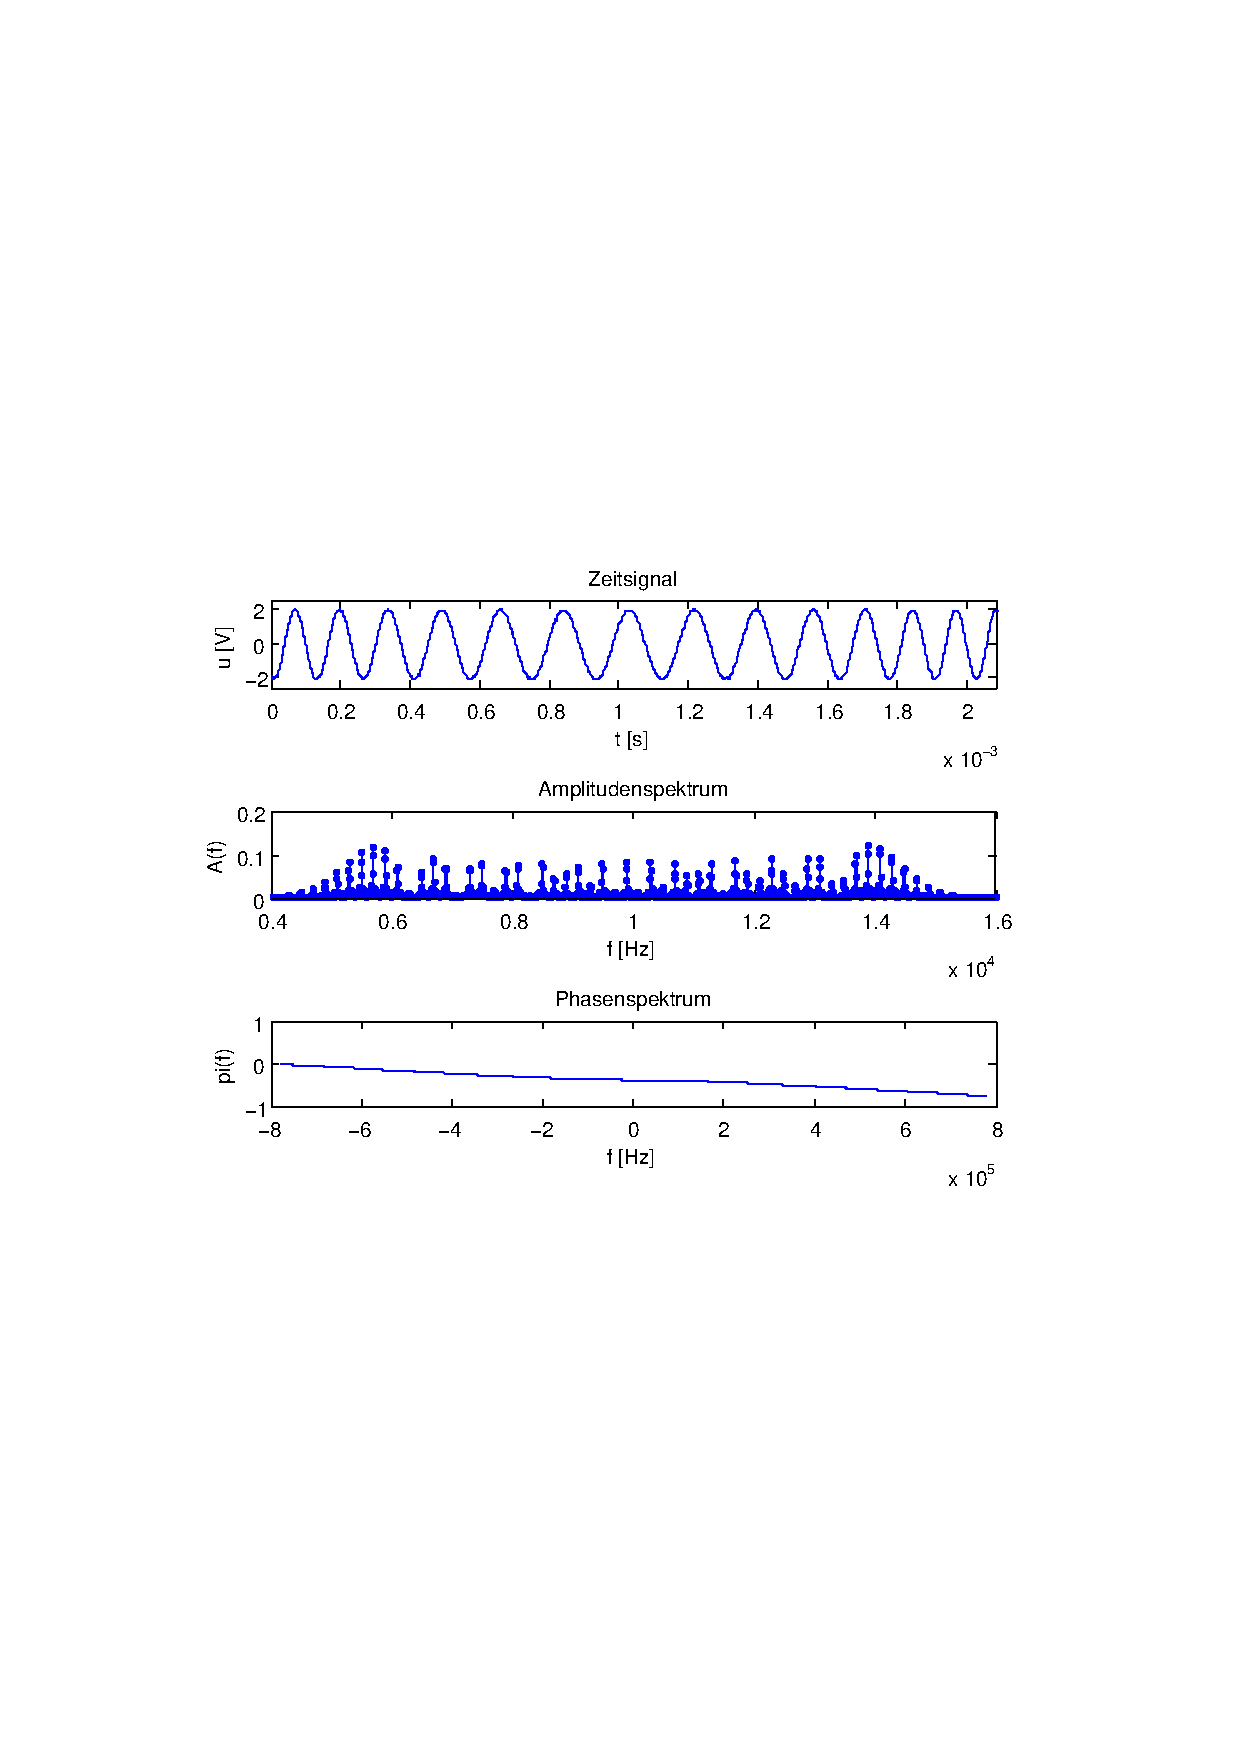
\includegraphics[scale=0.7, trim = 35mm 100mm 35mm 95mm, clip]{Bilder/f200_2}
                        \caption{FM von \SI{200}{\hertz} mit \SI{2}{\volt} Amplitude}
                    \end{figure}
                \end{minipage}
            
            \end{tabular}
            \end{center}            
        \end{quote}


        
        
        
        
    \end{quote}
    
    
    
    
    \subsection{Demodulation}
    \begin{quote}
        
        
        
        \begin{figure}[H]
			\begin{center}
			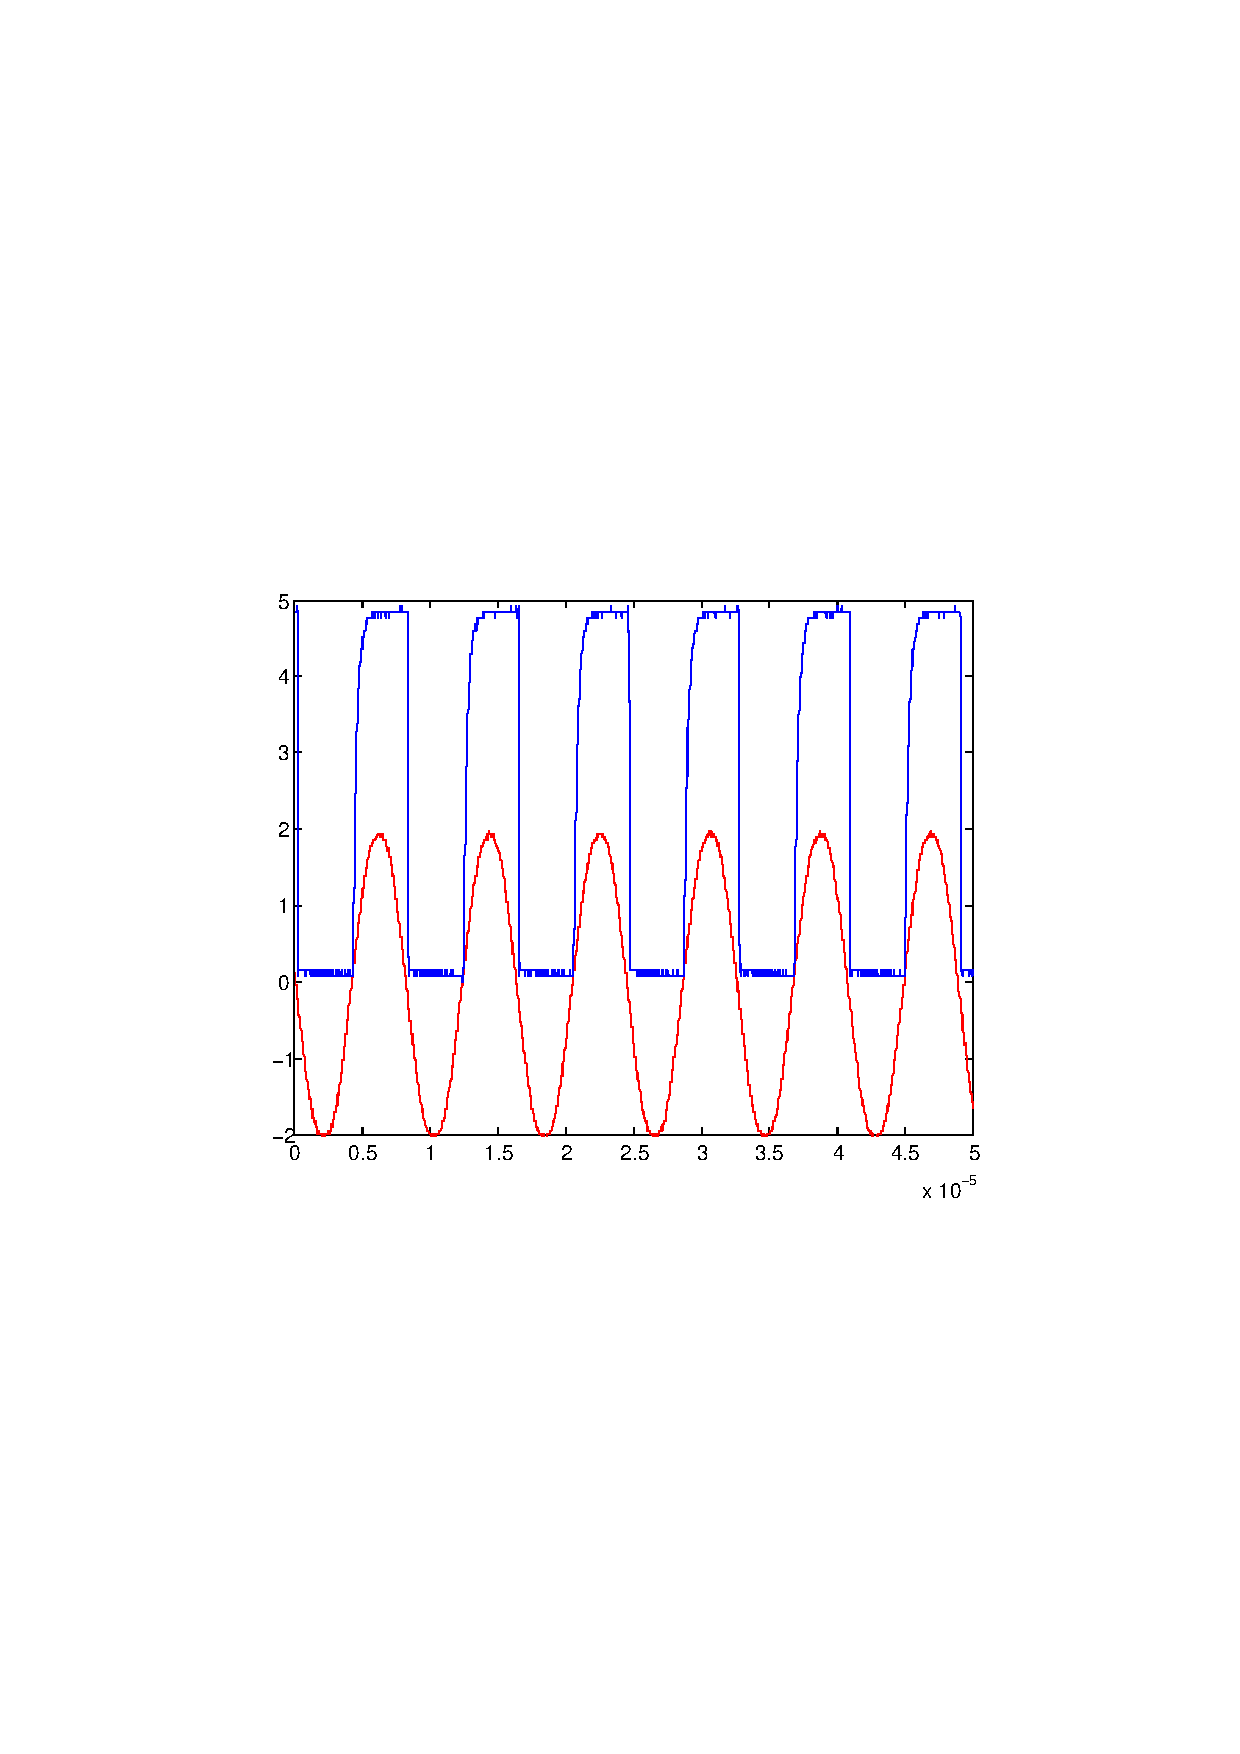
\includegraphics[scale=0.7, trim = 35mm 100mm 35mm 95mm,clip]{Bilder/spraFunktionsweiseComparator}
			\end{center}
		\caption{Funktionsweise des Komparators}
		\label{fig:fct Com}
	    \end{figure}
       
        In Abb. \ref{fig:TPGbreit} und \ref{fig:TPGschmal} ist der Ausgang des
        Twin Pulse Generator zu zwei unterschiedlichen Zeitpunkten zu sehen. Wie
        theoretisch erwartet, sind die Abstände zwischen den Pulsen je nach
        Frequenz des modulierten Signals unterschiedlich. 
        
         \begin{center}
            \begin{tabular}{ll}
            
            \hspace{-5cm}
                \begin{minipage}{0.67\textwidth}
                    \begin{figure}[H]
                        \label{fig:TPGbreit}
                        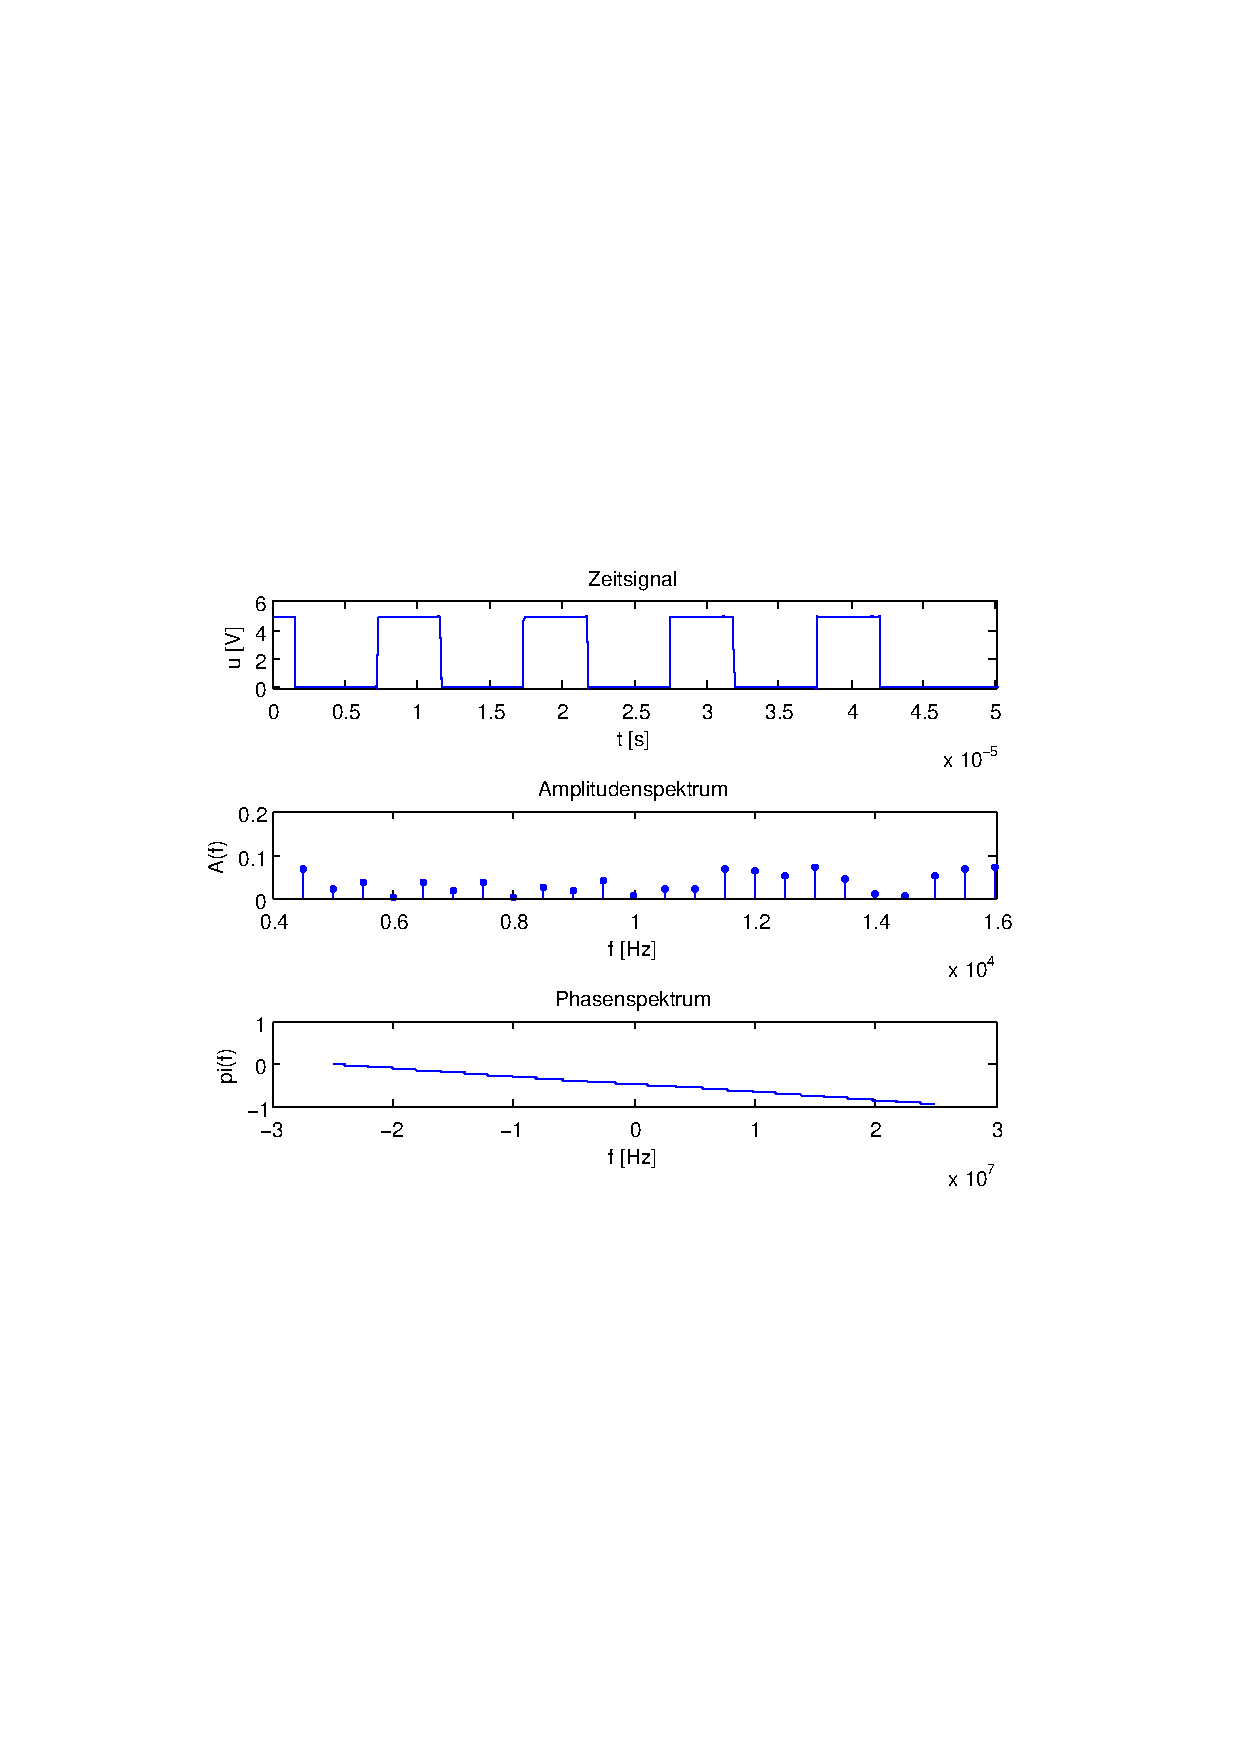
\includegraphics[scale=0.7, trim = 35mm 100mm 35mm 95mm, clip]{Bilder/f1TwPu_breit}
                        \caption{TPG breiter Abstände}
                    \end{figure}
                \end{minipage}
                
                \begin{minipage}{0.67\textwidth}
                    \begin{figure}[H]
                        \label{fig:TPGschmal}
                        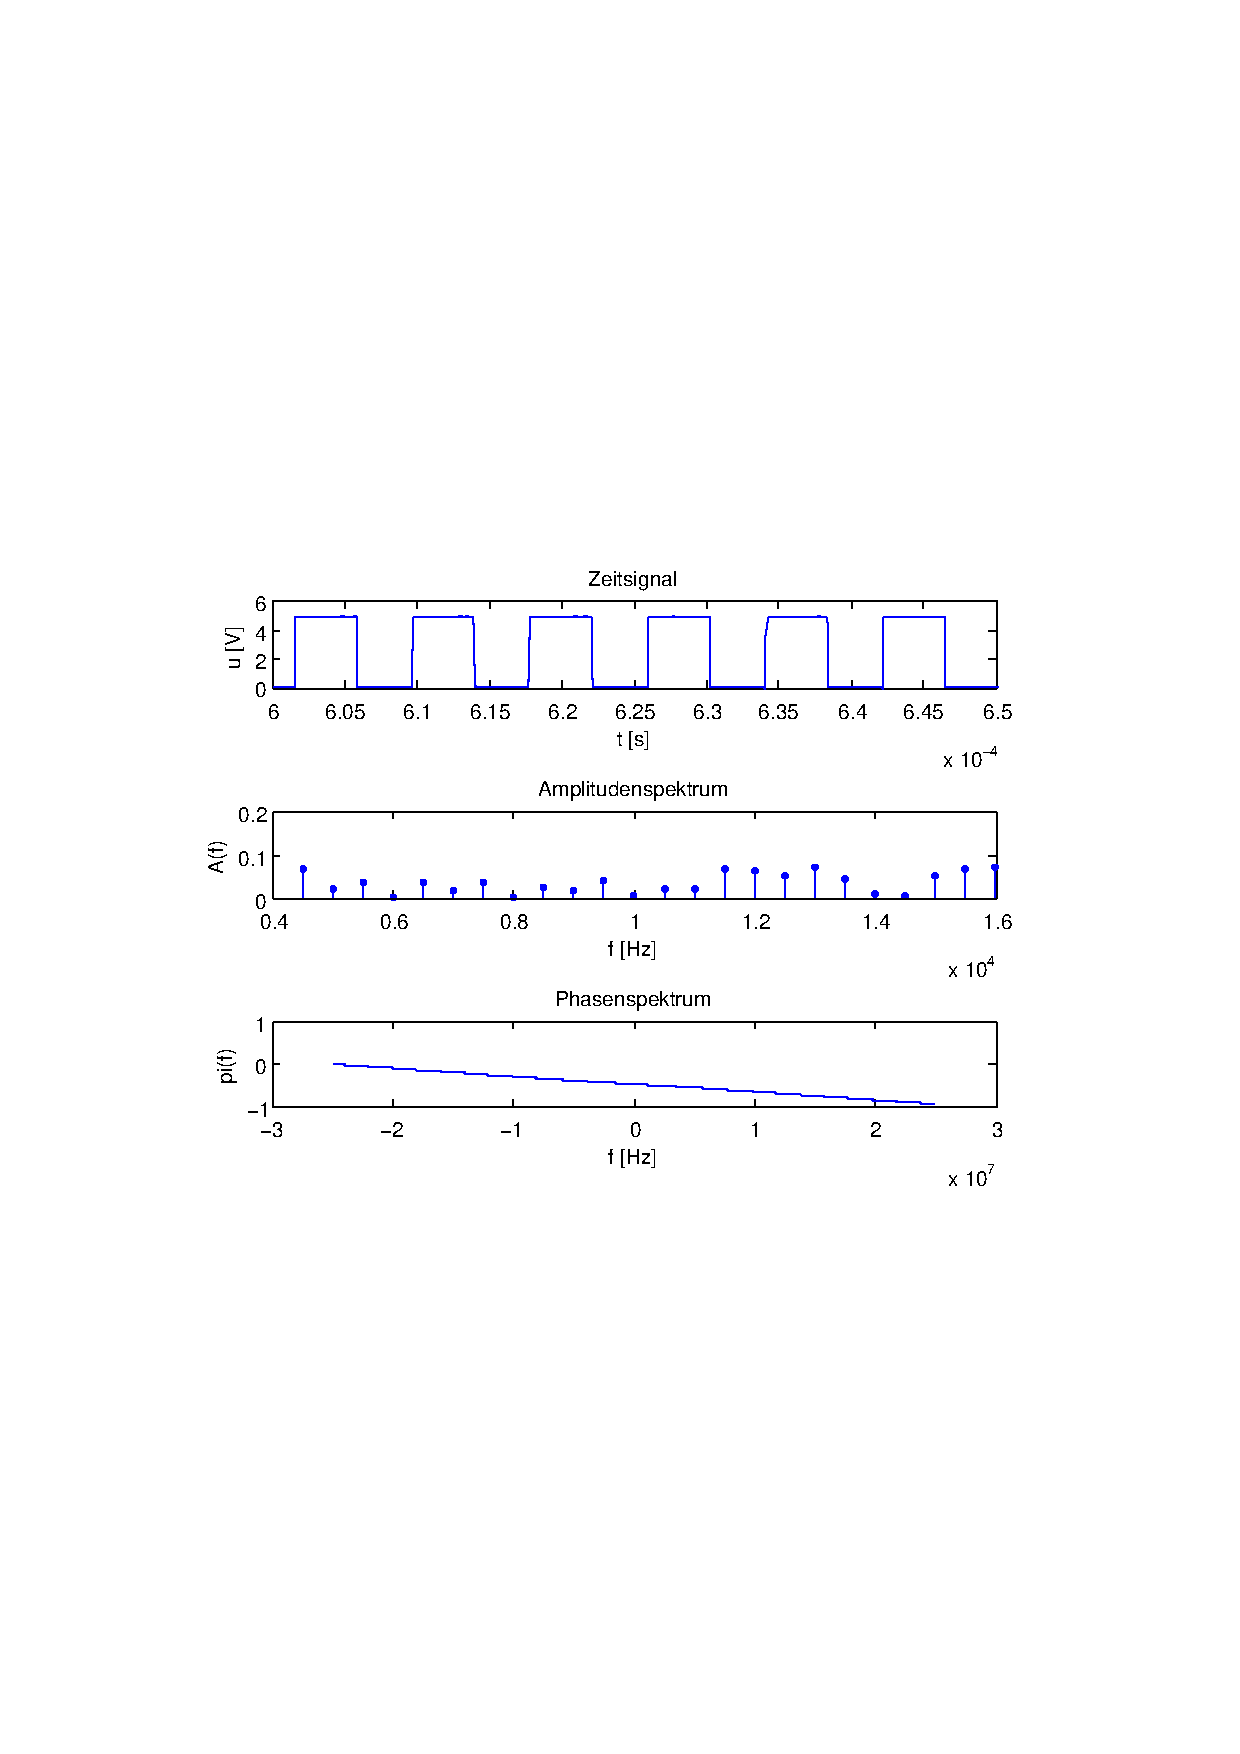
\includegraphics[scale=0.7, trim = 35mm 100mm 35mm 95mm, clip]{Bilder/f1TwPu_schmal}
                        \caption{TPG schmale Abstände}
                    \end{figure}
                \end{minipage}
            
            \end{tabular}
            \end{center}
          
          In den Abbildungen \ref{fig:vor Filter} und \ref{fig:nach Filter} kann
          man das Signal nach dem TPG und nach dem Komparator ohne den TPG
          erkennen. Die Signale sind nahezu gleich, nur, dass mit dem TPG das
          Signal eine idealere Rechteckform besitzt und die Pulse alle die
          gleiche Breite haben, aber unterschiedliche Abstände, wie oben
          besprochen.
            
         \begin{center}
            \begin{tabular}{ll}
            
            \hspace{-5cm}
                \begin{minipage}{0.67\textwidth}
                    \begin{figure}[H]
                        \label{fig:vor Filter}
                        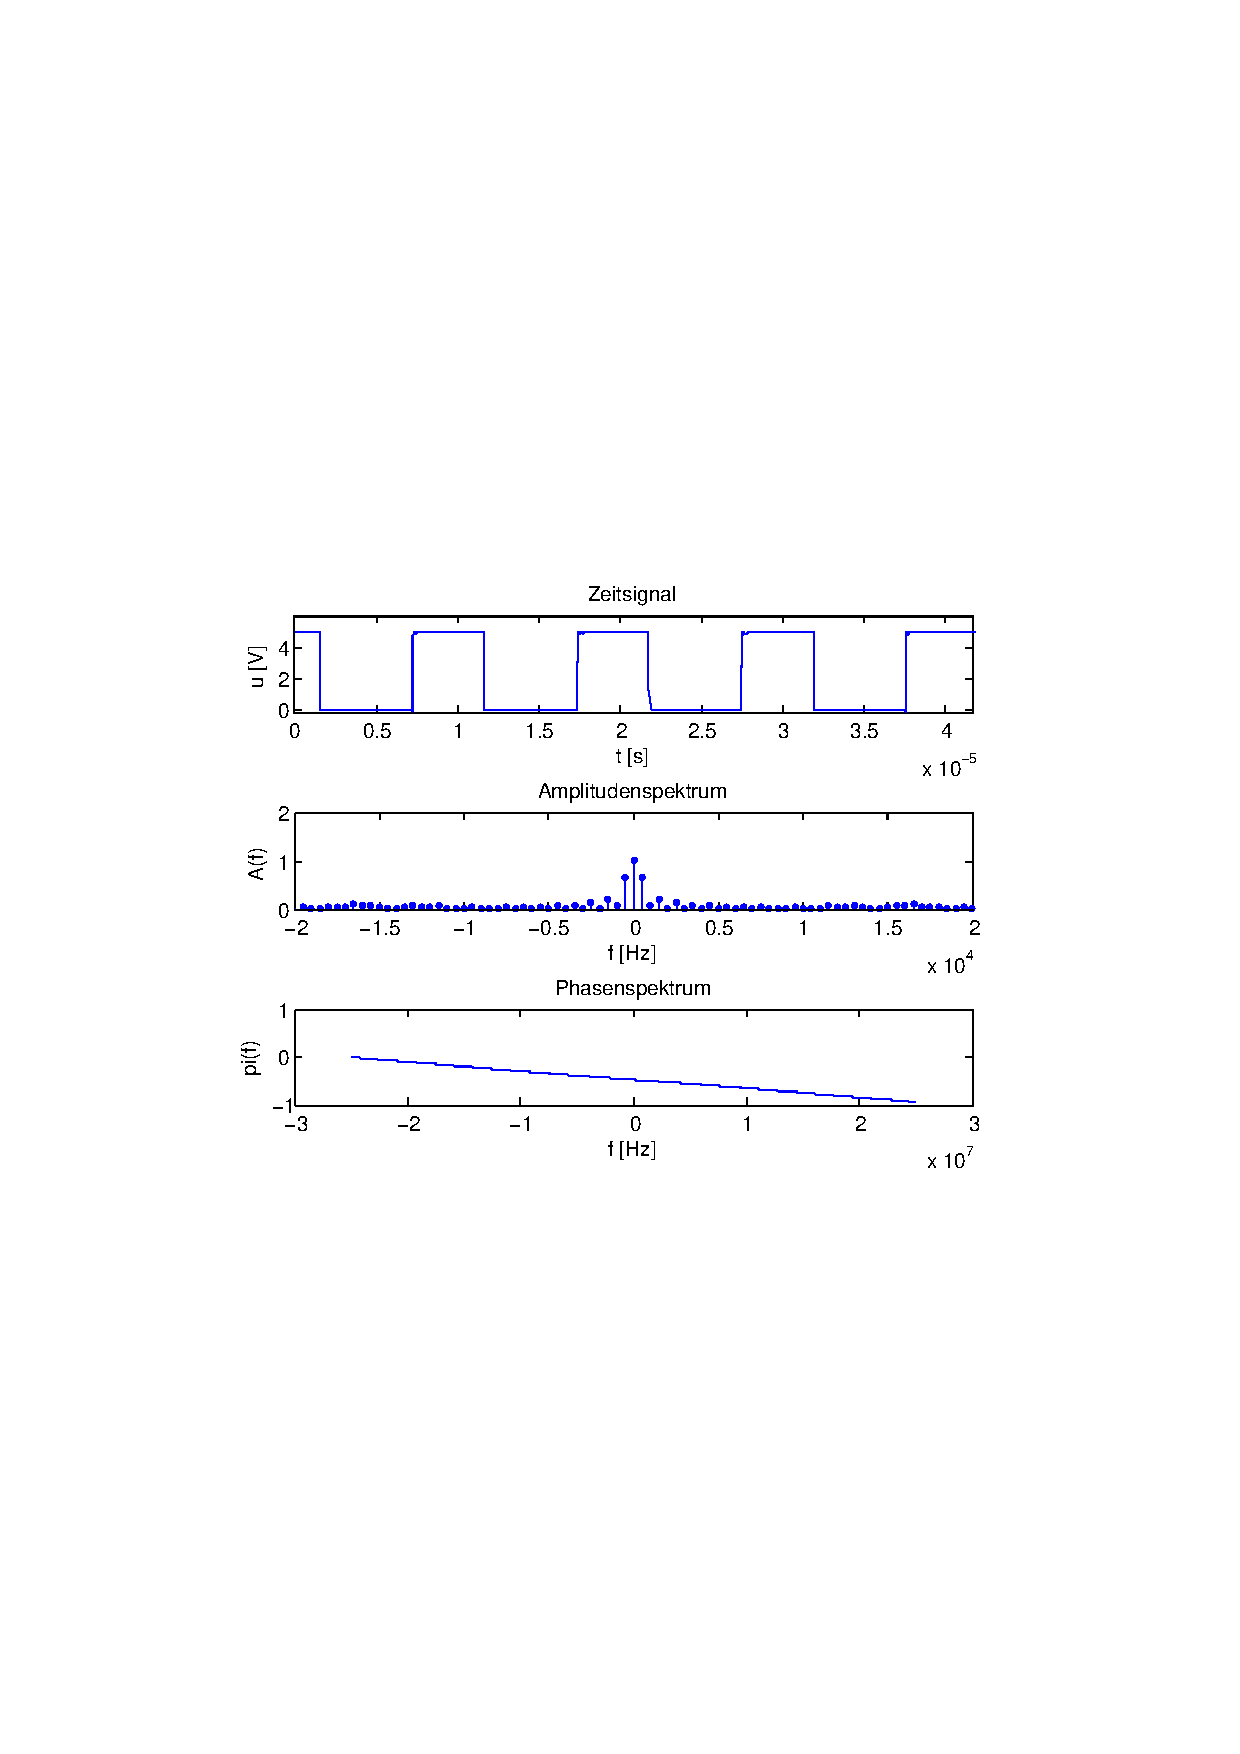
\includegraphics[scale=0.7, trim = 35mm 100mm 35mm 95mm, clip]{Bilder/TwPuB}
                        \caption{Nach dem TPG}
                    \end{figure}
                \end{minipage}
                
                \begin{minipage}{0.67\textwidth}
                    \begin{figure}[H]
                        \label{fig:nach Filter}
                        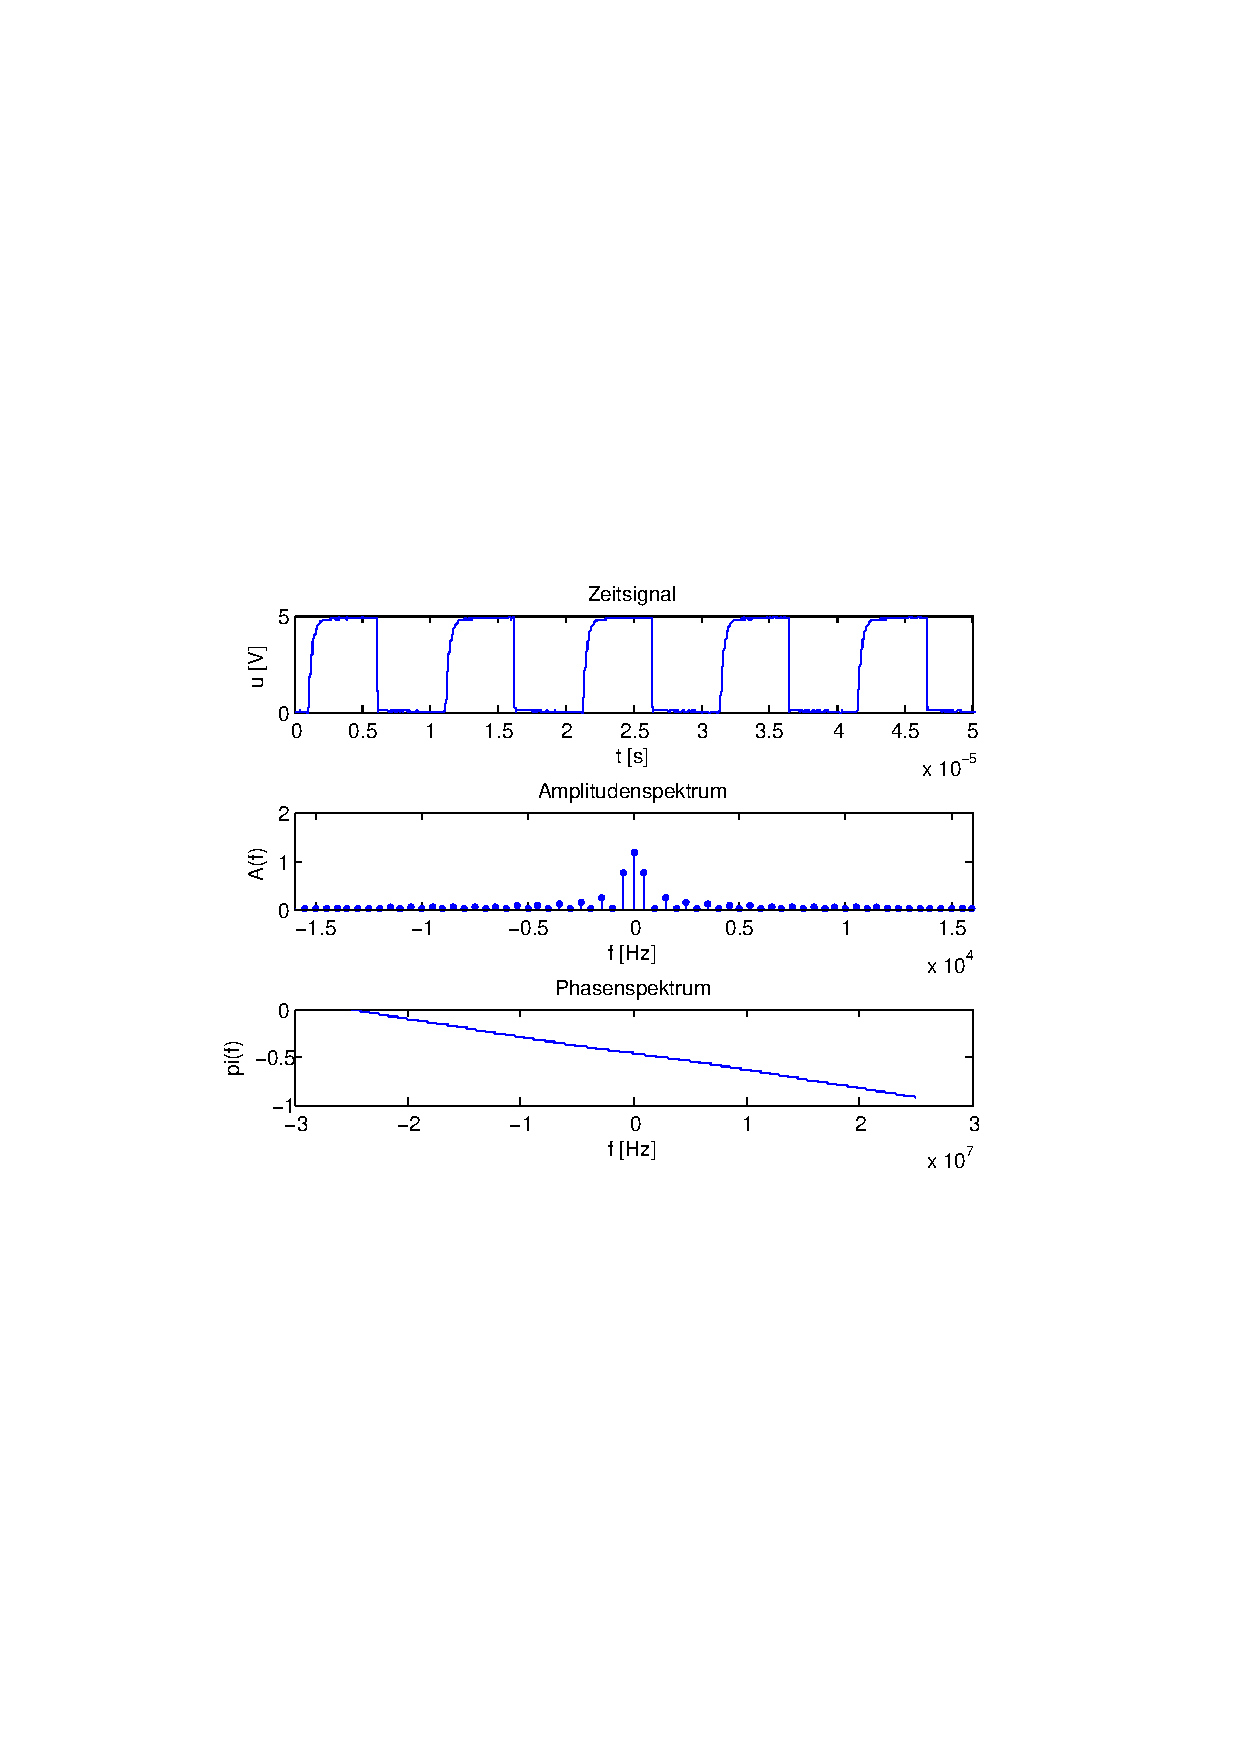
\includegraphics[scale=0.7, trim = 35mm 100mm 35mm 95mm, clip]{Bilder/f1comp}
                        \caption{Nach dem Komparator ohne TPG}
                    \end{figure}
                \end{minipage}
            
            \end{tabular}
            \end{center}
        
        Zuletzt ist in Abb. \ref{fig:filter} das tiefpass-gefilterte
        Signal zu erkennen, das dann dem demodulierten Signal, also dem
        Nutzsignal entsprechen soll. Auffällig ist, dass das Signal im Vergleich
        zu Demodulation bei der AM deutlich abweicht vom eigentlich gesendeten
        Signal. 
        
        \begin{figure}[H]
			\begin{center}
			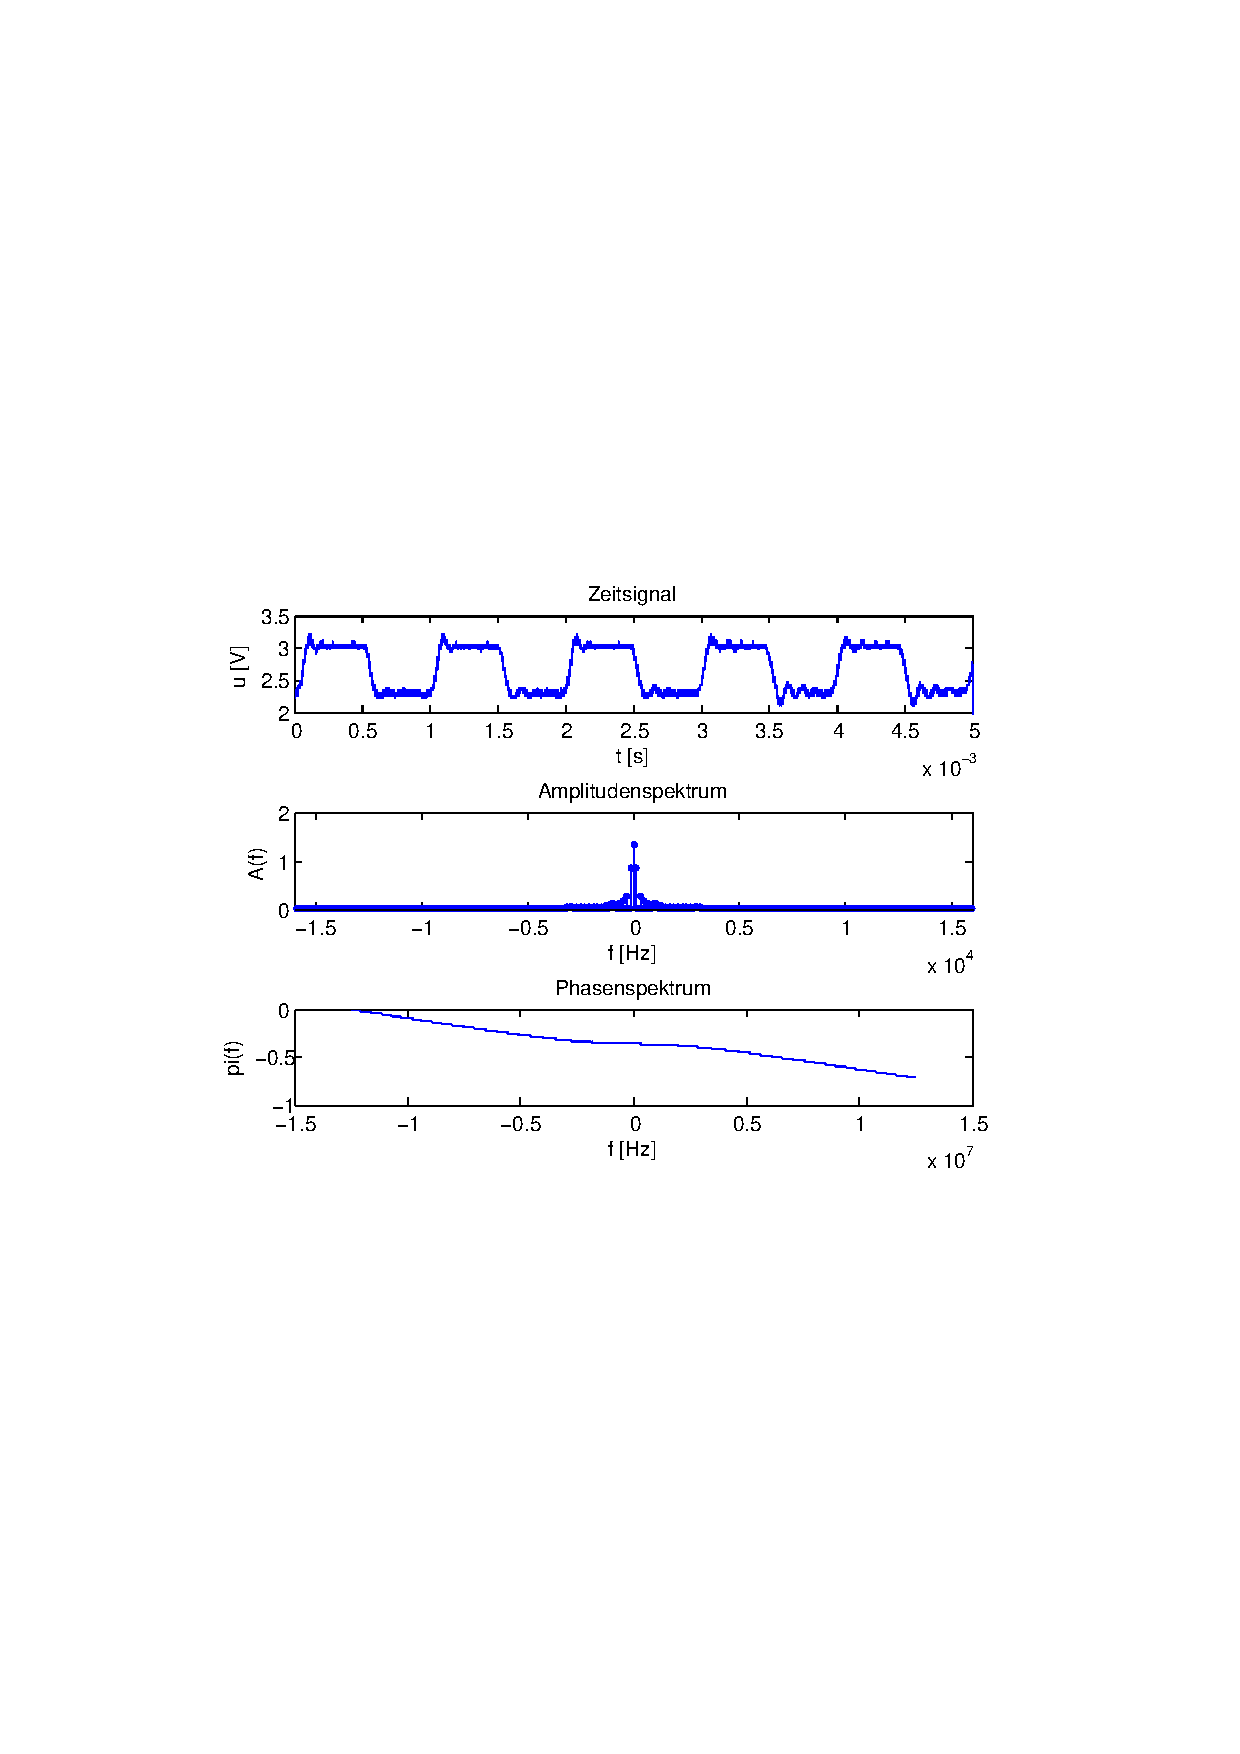
\includegraphics[scale=0.7, trim = 35mm 100mm 35mm 95mm,clip]{Bilder/f1filB}
			\end{center}
		\caption{demoduliertes Signal}
		\label{fig:filter}
	    \end{figure}
        
        frequenzhub
        trägerfrequenz
        signalfrequenz
        $\beta$
        Basisband
       
        
    \end{quote}
    
\end{quote}



% \begin{quote}
%     \lstinputlisting[
%         caption={Scilab-script},
%         label=lst:scilab]
%         {./Scilab/Motor.sce}
%         
% \end{quote}

%--------------------------------------------------------------------
%--------------------------------------------------------------------
% \begin{thebibliography}{999}
% 
% \bibitem{Boris}Boris Henckell: Ein Paar sachen geklaut.. ähhh inspirationen geholt
% \href{http://www.krachler.com/fileadmin/user_upload/arbeiten/Reglersynthese_Christian_Krachler.pdf}{Reglersynthese nach dem Frequenzkennlinienverfahren}, S16, S22, 08.05.2012
% 
% 
% %Name, Vorname.; evtl. Name2, Vorname2.: Titel des Dokumentes
% %oder Buches, Zeitschrift/Verlag/URL (Auflage, Erscheinungsort, -jahr), ggf. Seitenzahlen
% %\bibitem [Wiki10] {DigitaleMesskette2} \url{www.wikipedia.org}, Zugriff 22.03.2010
% \end{thebibliography}


\end{document}
